\documentclass[12pt]{article}
\usepackage{amsmath}
\usepackage{amssymb}
\usepackage{amsthm}
\usepackage{accents}
\usepackage{graphicx}
\usepackage{listings}
\usepackage[framed,numbered,autolinebreaks,useliterate]{mcode}
\setlength{\oddsidemargin}{0in}
\setlength{\textwidth}{6.5in}
\setlength{\topmargin}{-.55in}
\setlength{\textheight}{9in}
\pagestyle{empty}
\renewcommand \d{\displaystyle}
\begin{document}
\noindent Stephanie Klumpe

\noindent Math 6680

\noindent HW 2

5.1.Modify Program 9 to compute and plot the maximum error over $[-1,1]$ for equispaced and Chebyshev interpolation on a log scale as a function of N. What asymptotic divergence and convergence constants do you observe for these two cases? (Confine your attention to small enough values of $N$ that rounding errors are not dominant.) Now, based on the potential theory of this chapter, determine exactly what these geometric constants should be. How closely do your numerical experiments match the theoretical answers?
\footnote{I accidentally did this problem and didn't want to delete all of the work, so I kept it in.}\\\\

Here, we are choosing $N$ to be multiples of 4 between 4 and 28.\\
\begin{figure}[htp]
\centering
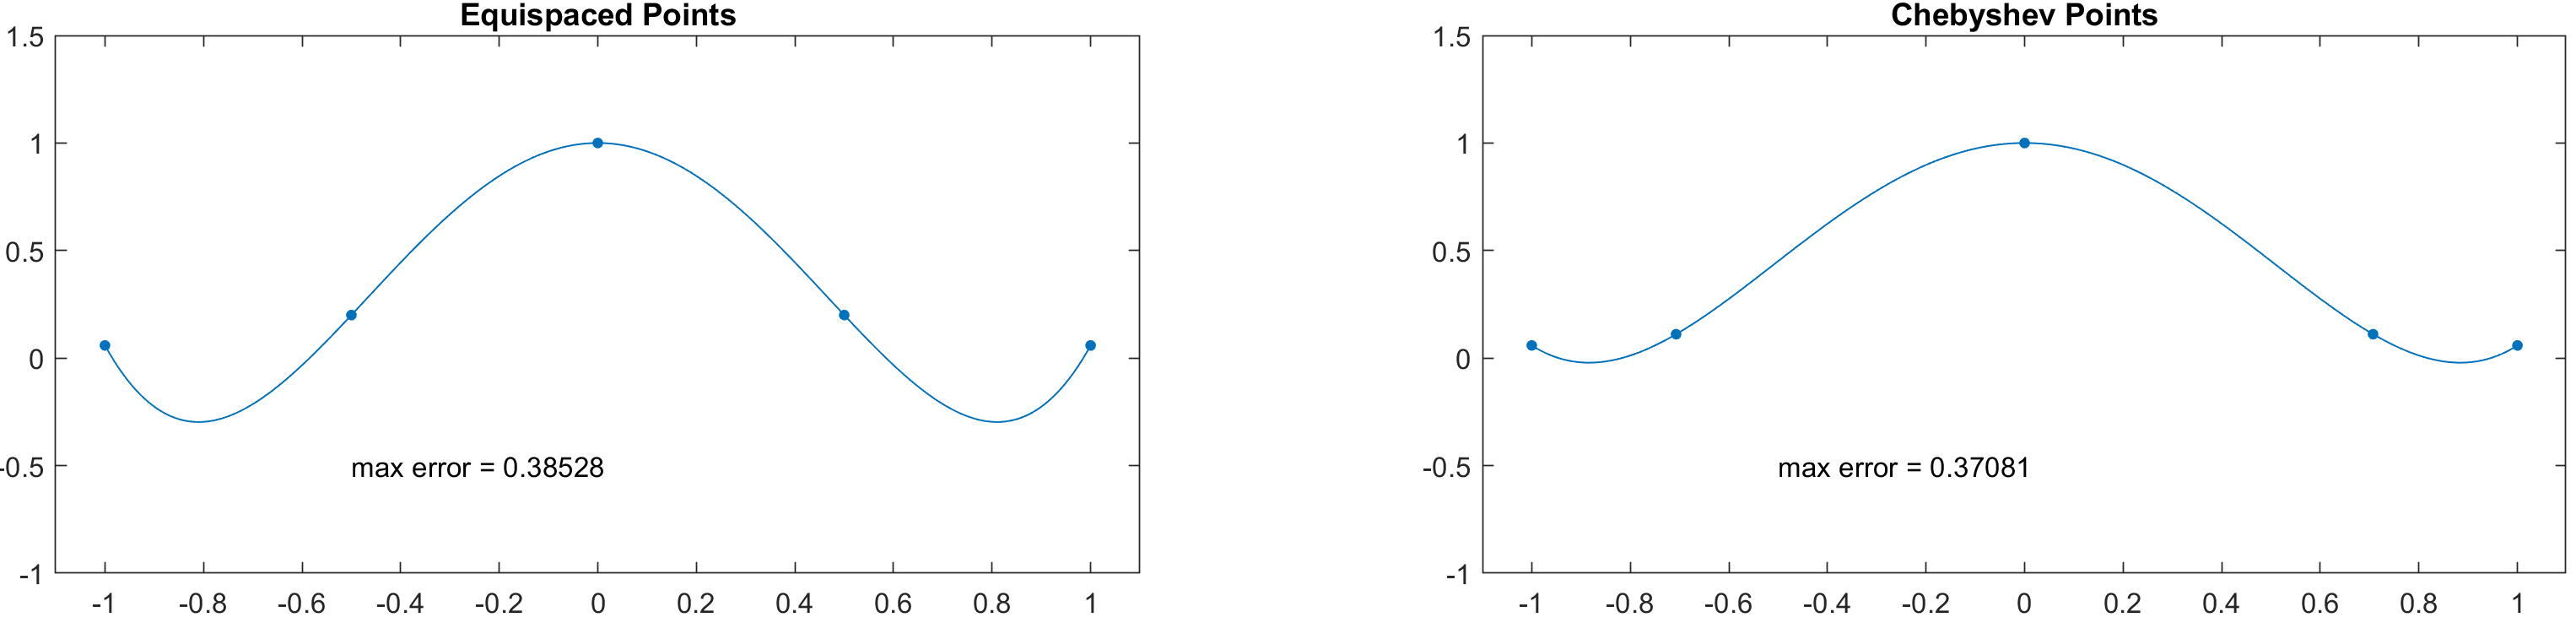
\includegraphics[scale=0.2]{5_14.PNG}
\caption{$N=4$}
\end{figure}
\begin{figure}[htp]
\centering
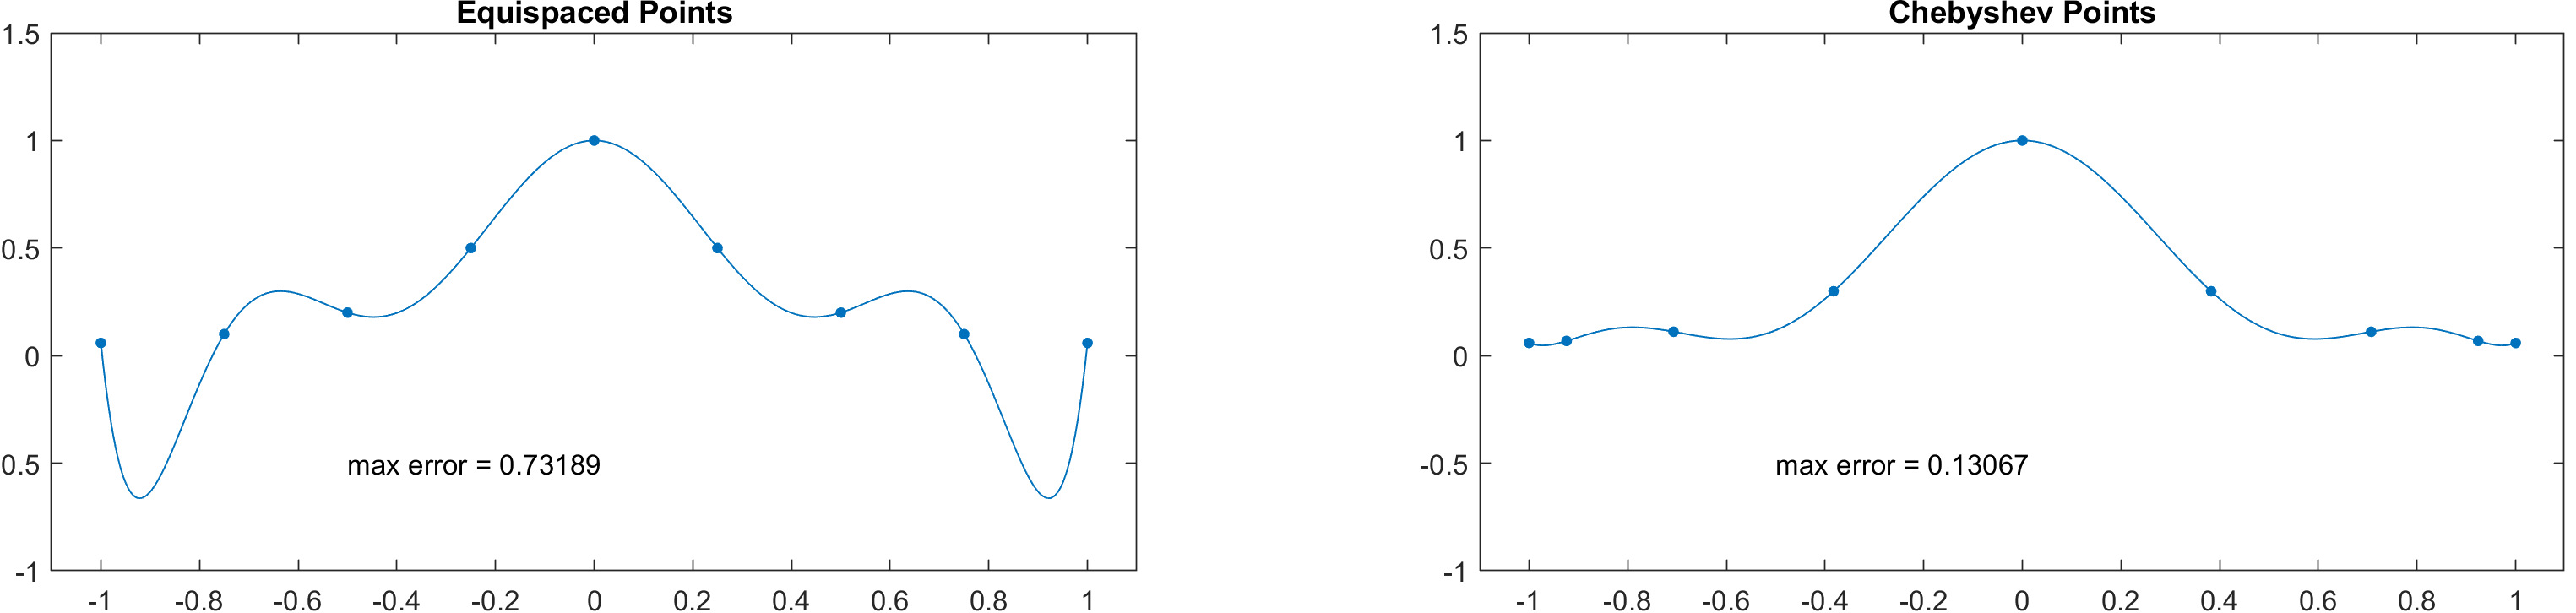
\includegraphics[scale=0.2]{5_18.PNG}
\caption{$N=8$}
\end{figure}
\begin{figure}[htp]
\centering
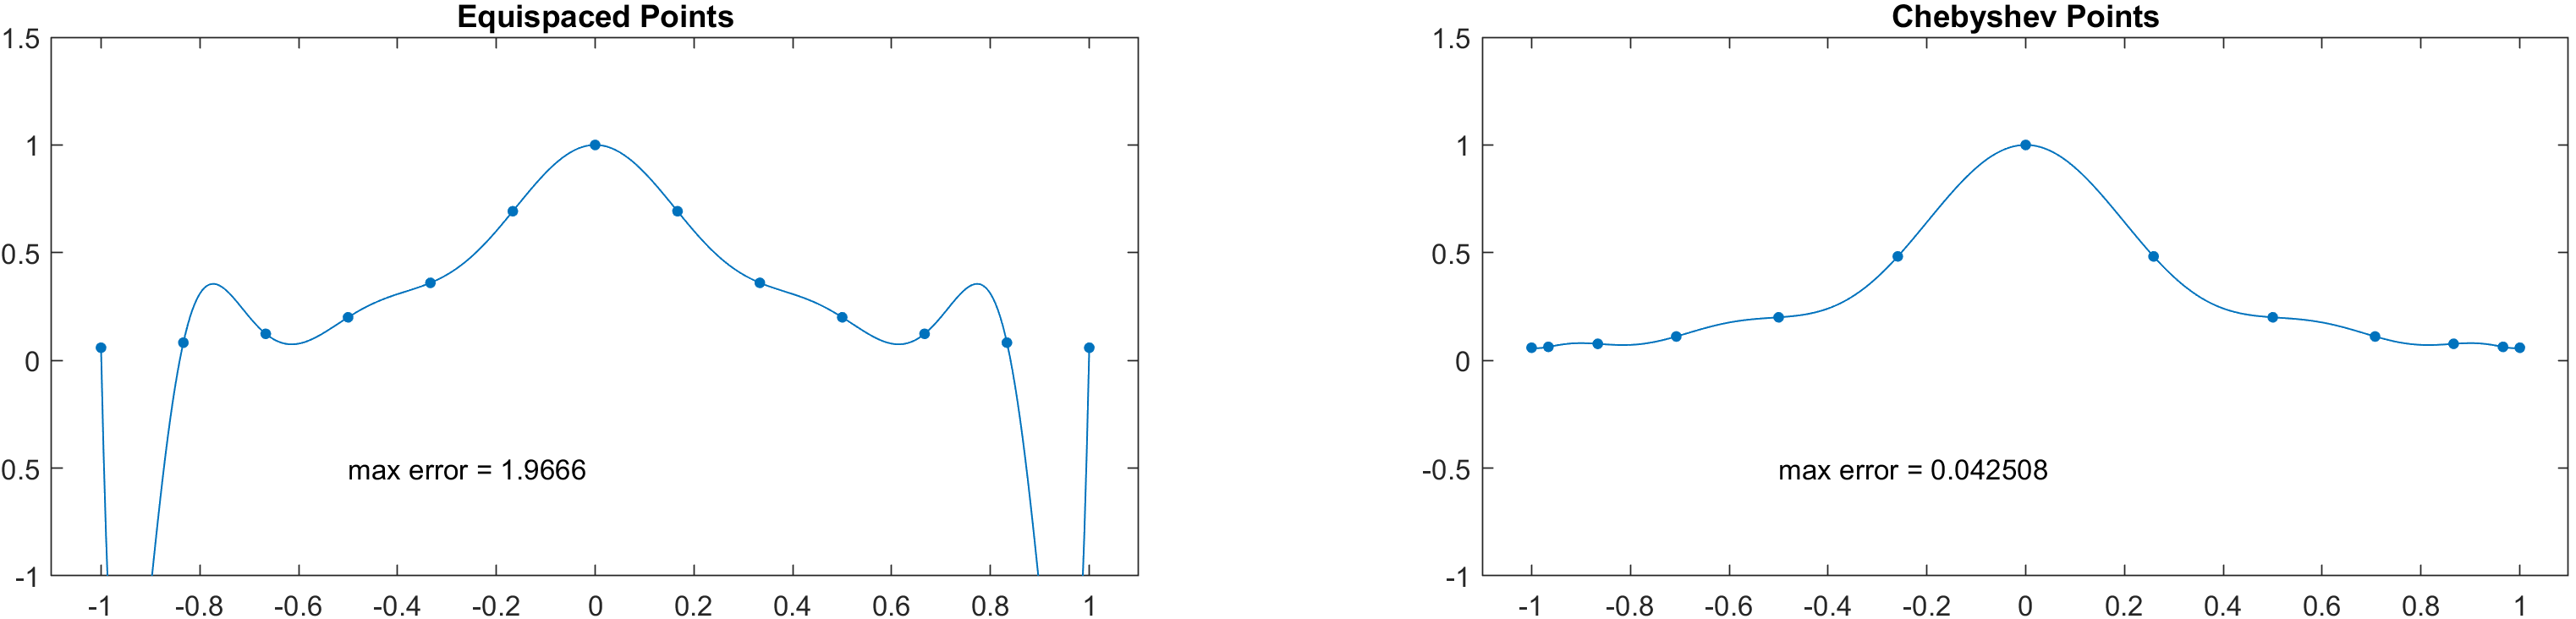
\includegraphics[scale=0.2]{5_112.PNG}
\caption{$N=12$}
\end{figure}
\begin{figure}[htp]
\centering
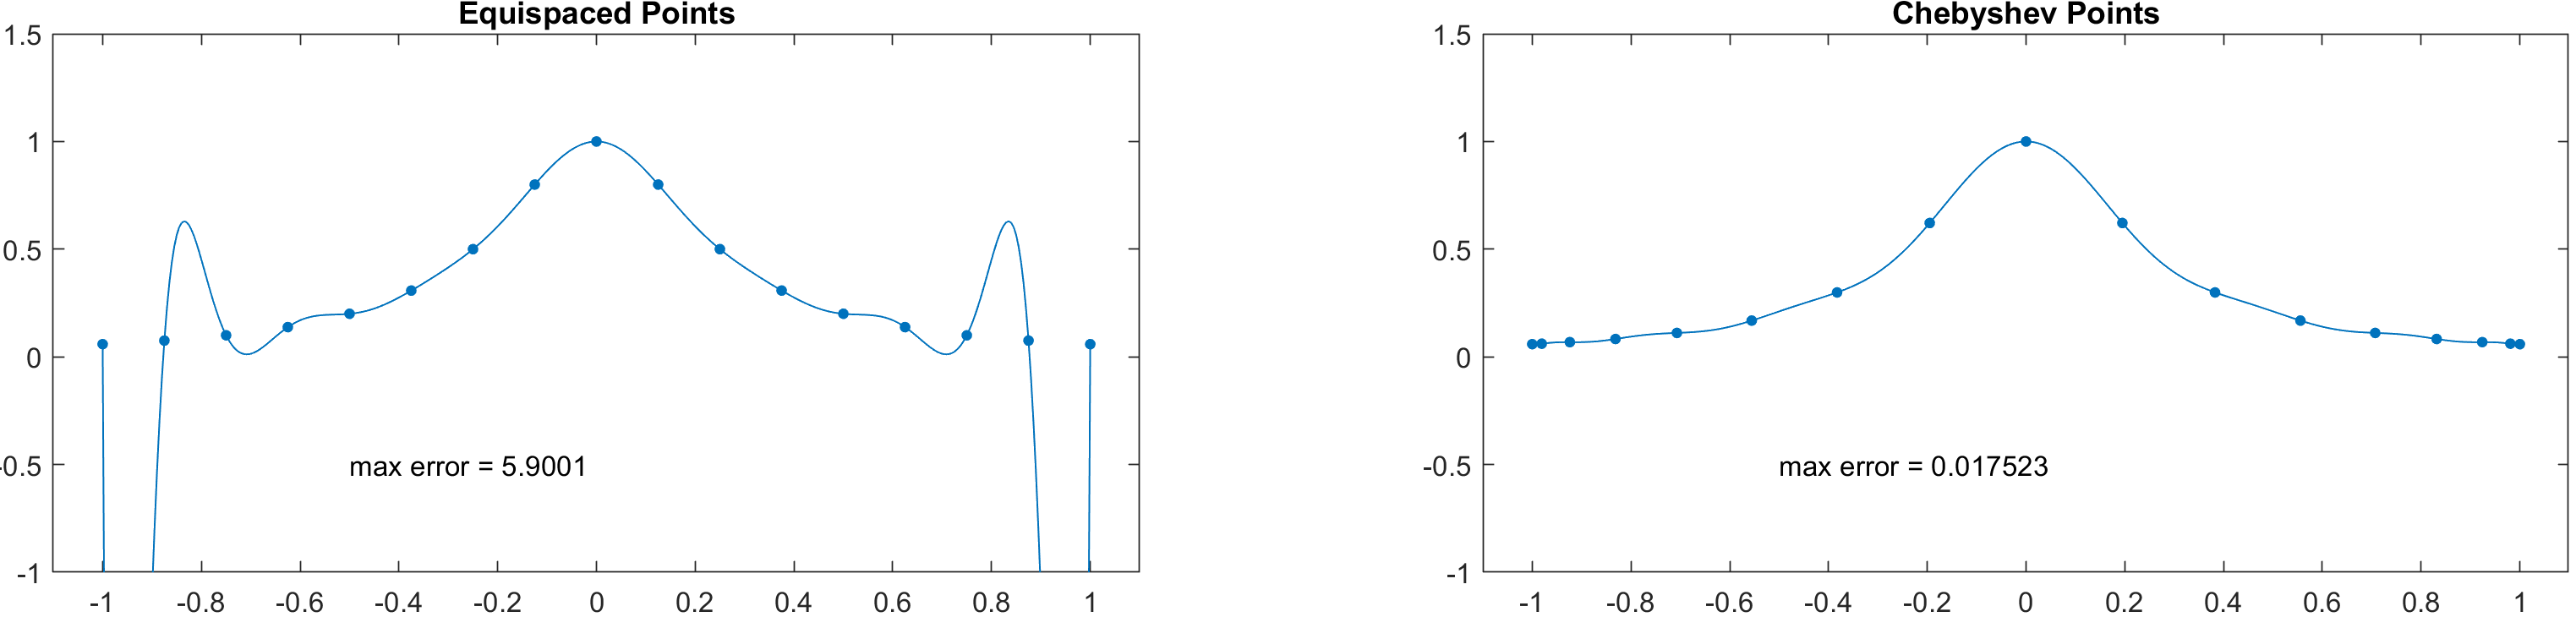
\includegraphics[scale=0.2]{5_116.PNG}
\caption{$N=16$}
\end{figure}
\begin{figure}[htp]
\centering
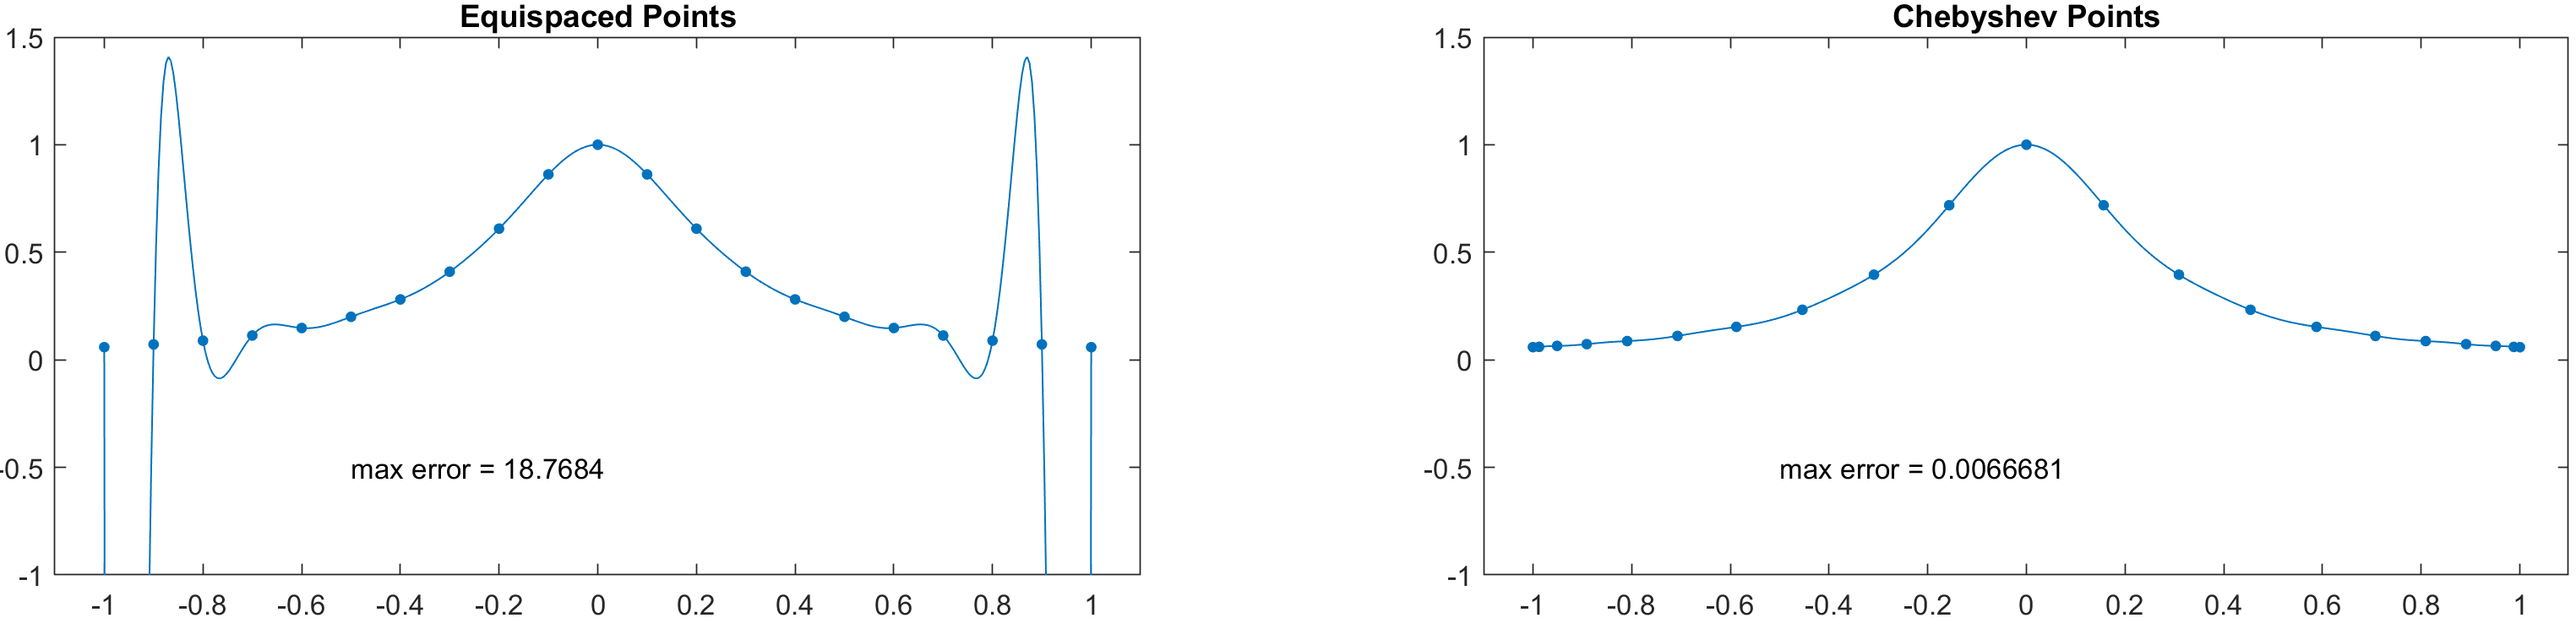
\includegraphics[scale=0.2]{5_120.PNG}
\caption{$N=20$}
\end{figure}
\begin{figure}[htp]
\centering
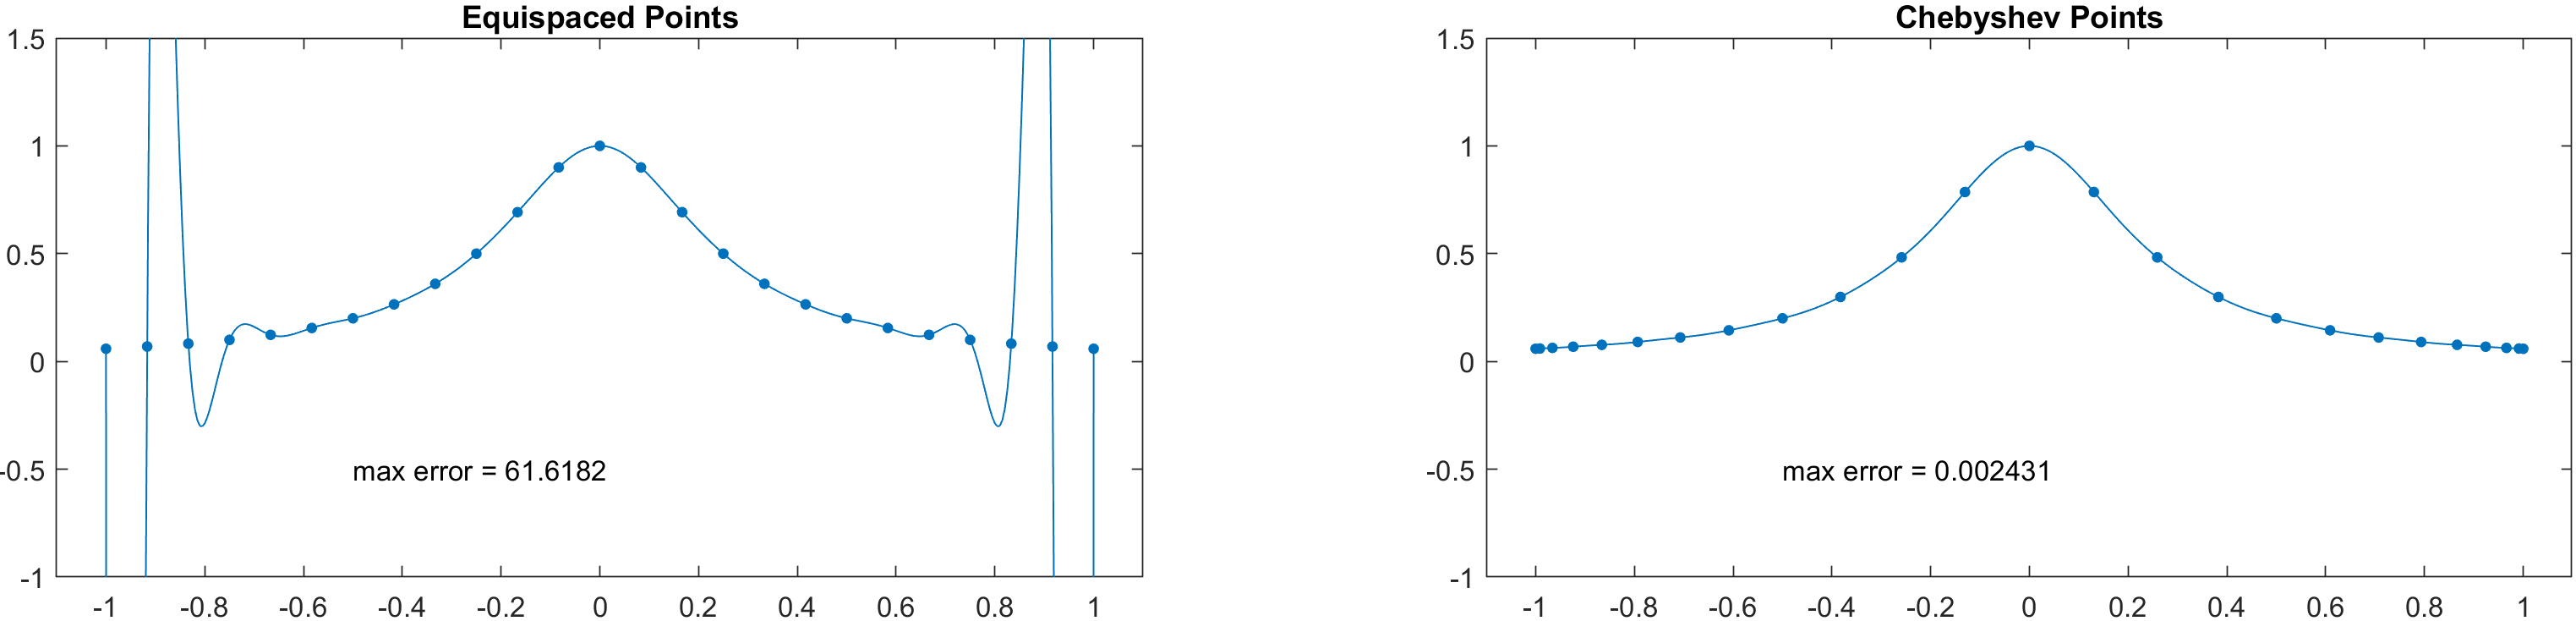
\includegraphics[scale=0.2]{5_124.PNG}
\caption{$N=24$}
\end{figure}
\begin{figure}[htp]
\centering
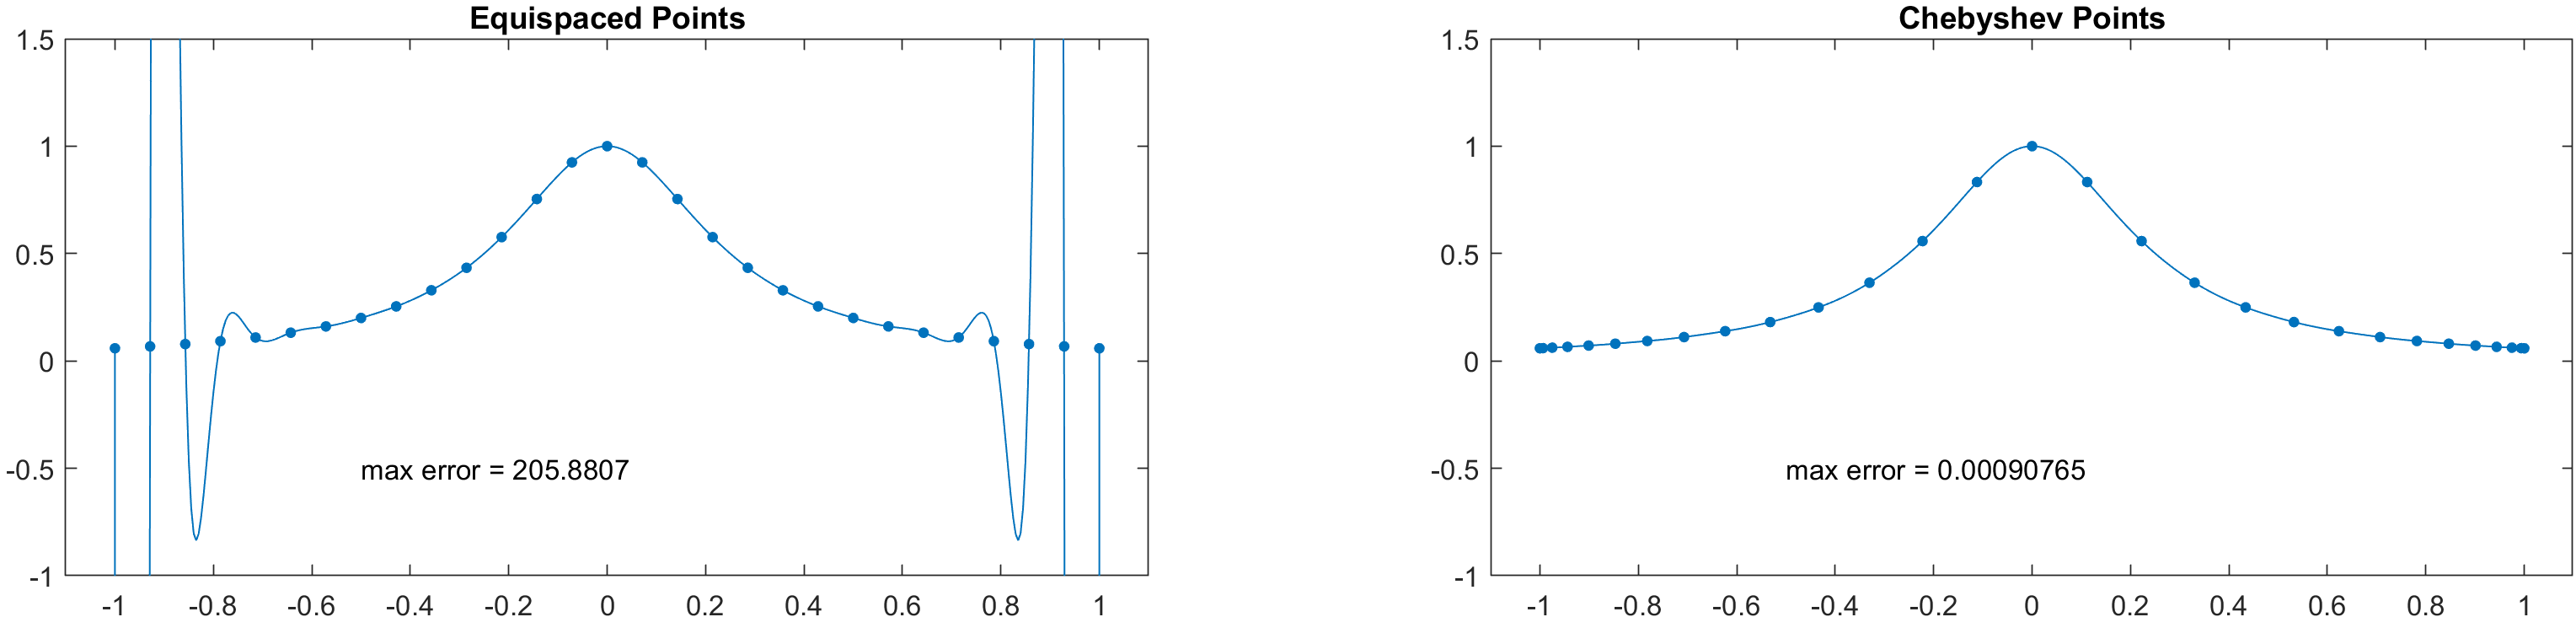
\includegraphics[scale=0.2]{5_128.PNG}
\caption{$N=28$}
\end{figure}

\newpage

Now, looking at the two plots of the error vs $N$, we see that for the equidistal points, there is no convergence. Rather, there is divergence towards infinity and this divergence happens exponentialy. Similarly, for the Chebyshev nodes, there is an exponential plotting, however, this is exponentially convergent.\\

\begin{figure}[htp]
\centering
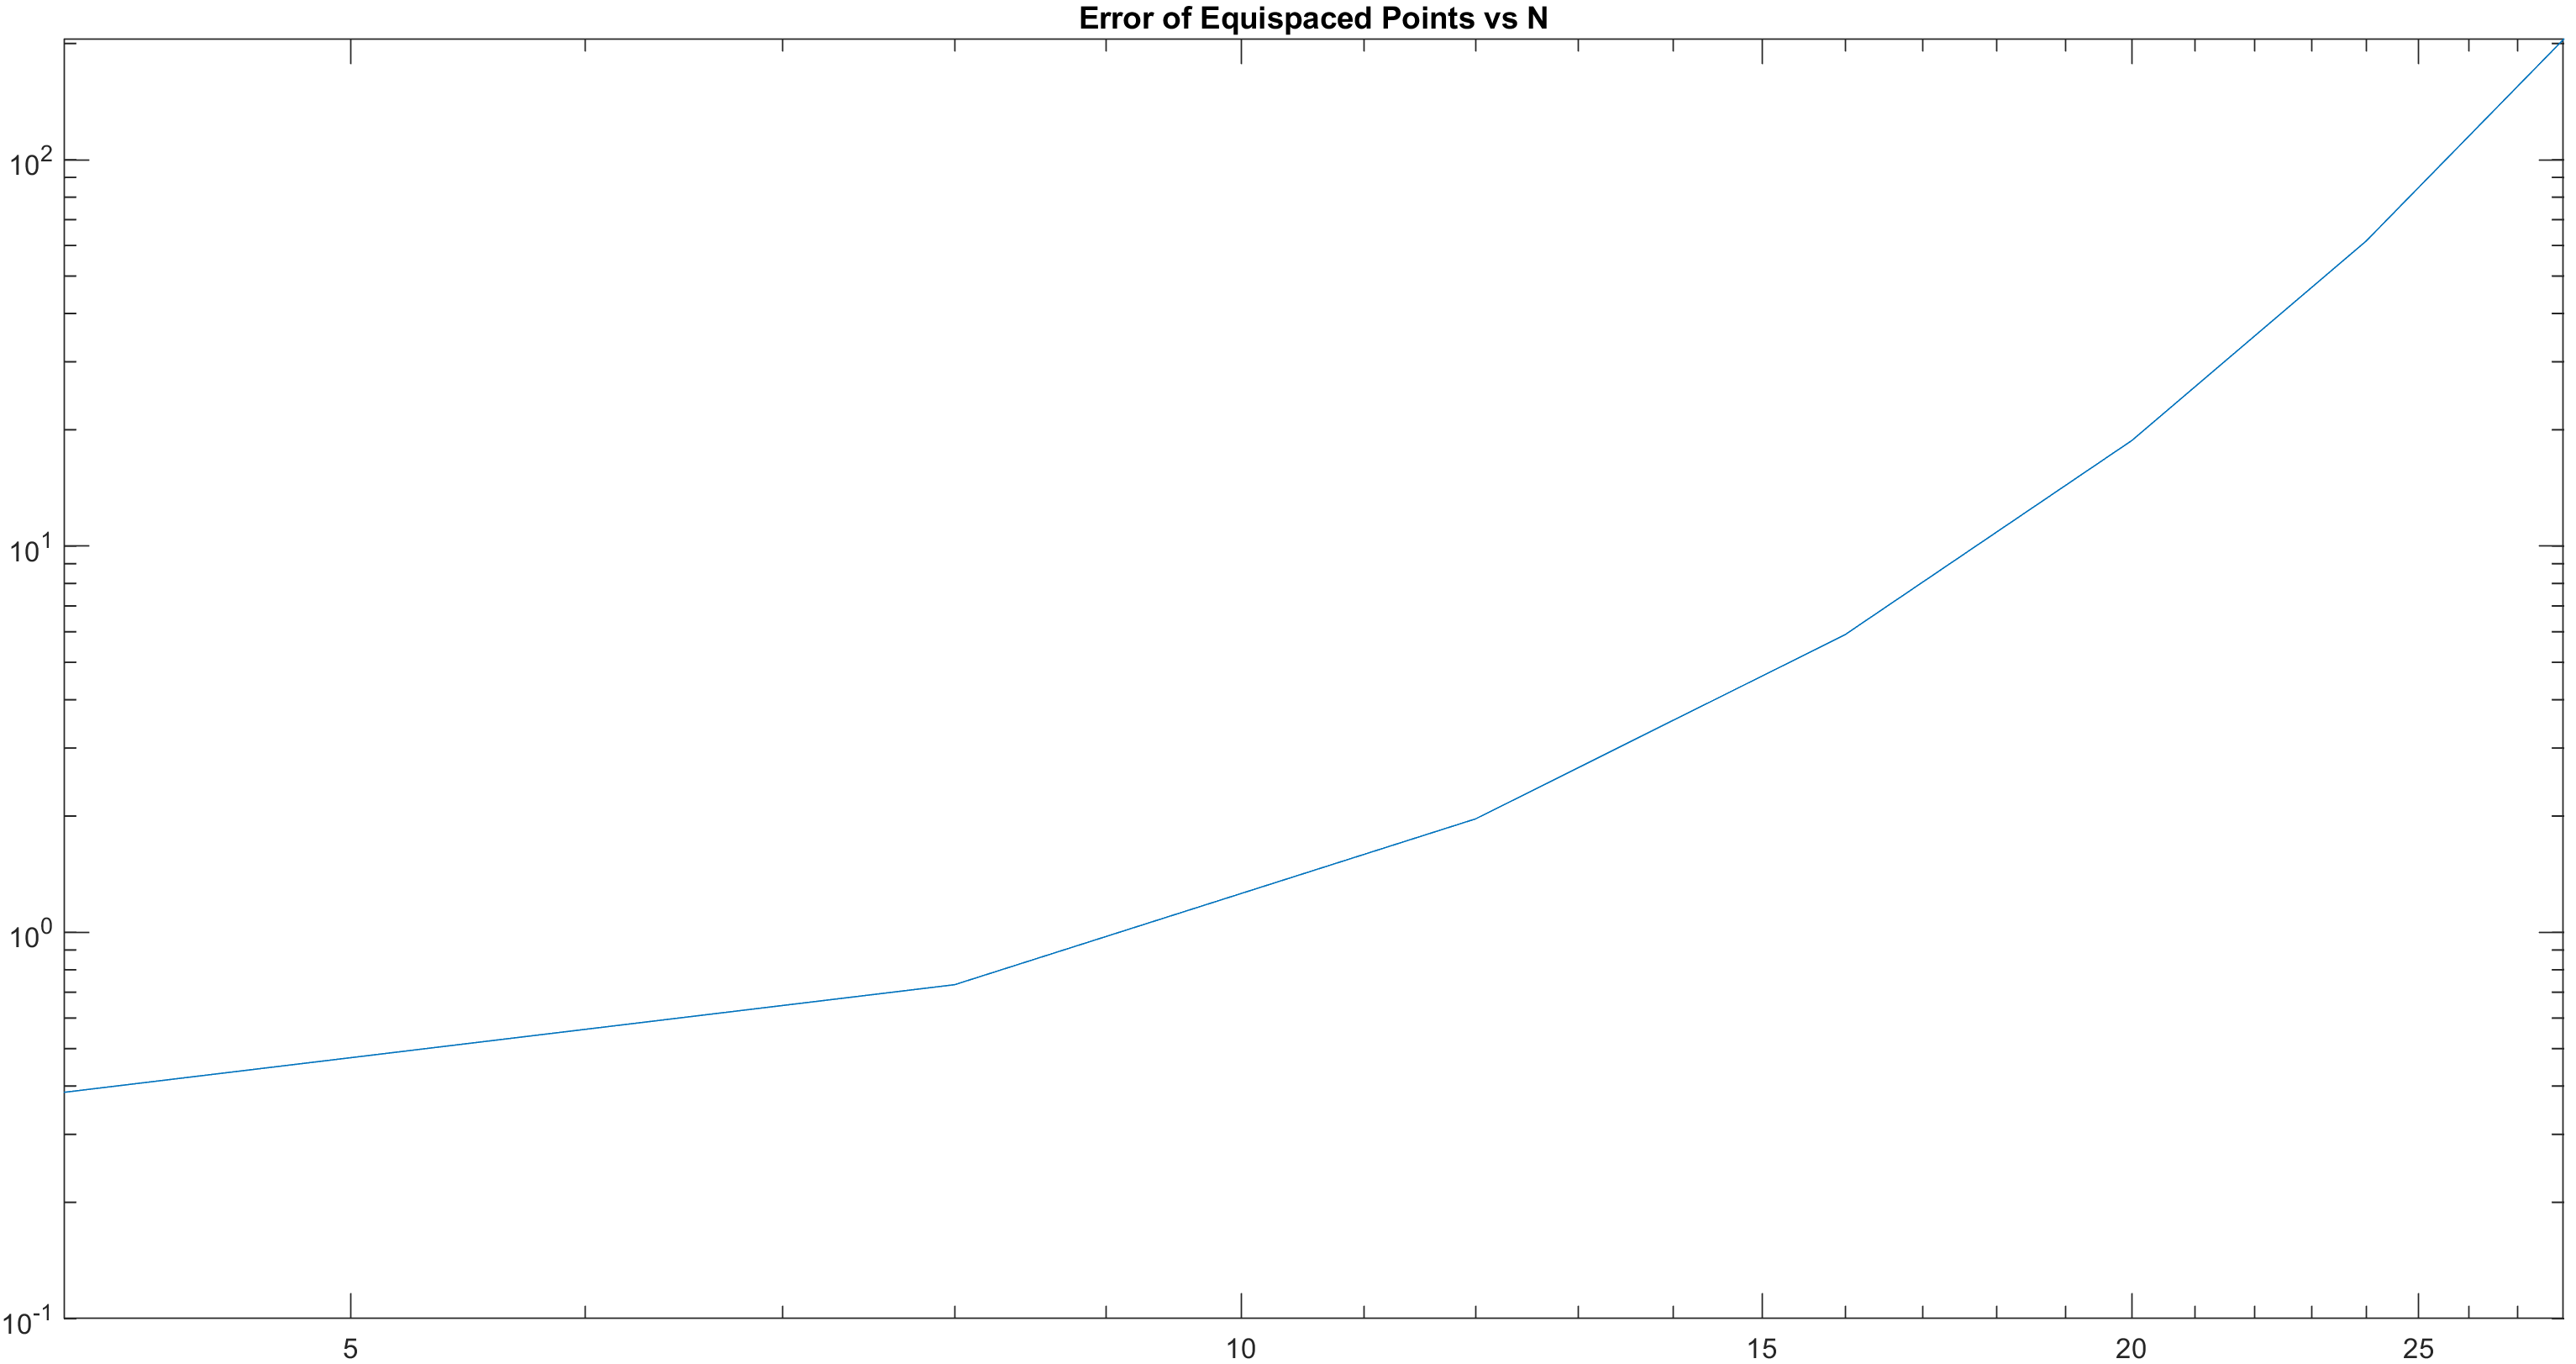
\includegraphics[scale=0.12]{5_1equi.PNG}
\end{figure}
\begin{figure}[htp]
\centering
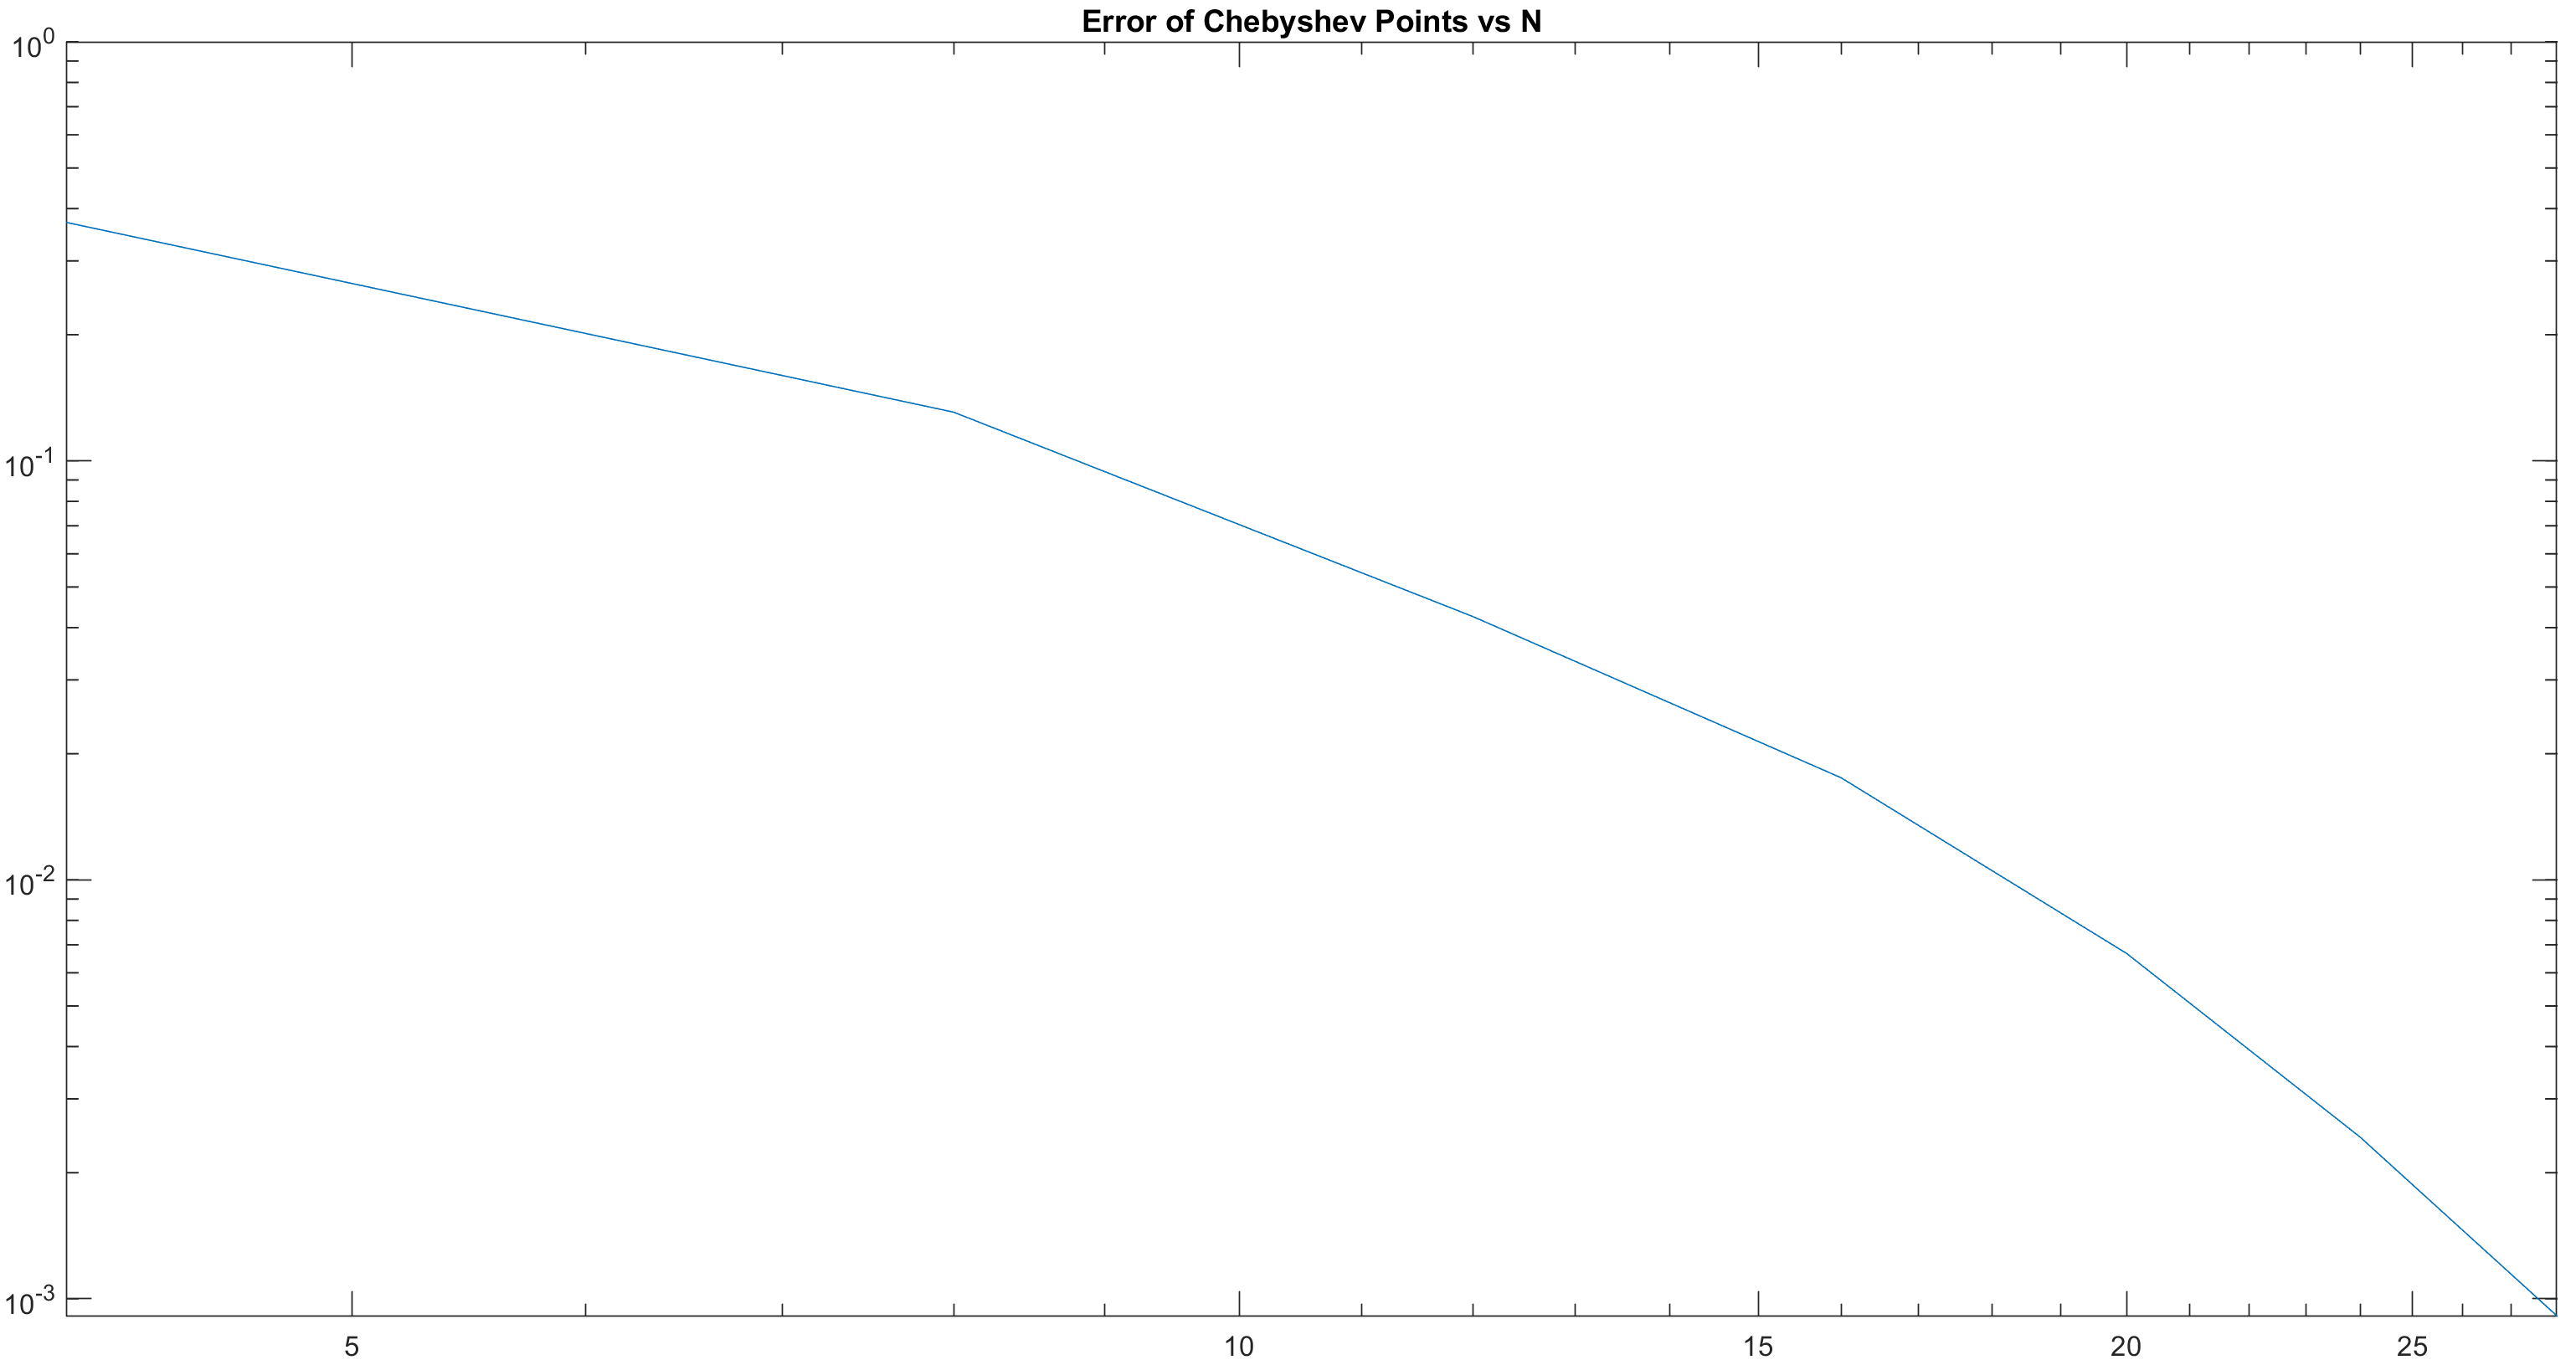
\includegraphics[scale=0.12]{5_1cheb.PNG}\\
\end{figure}

\newpage
\lstinputlisting{problem5_1.m}
\newpage

\newpage

5.3. Let $E_N = \inf_p||p(x)-e^x||_{\infty}$, where $||f||_{\infty}=\sup_{x\in[-1,1]}|f (x)|$, denote the error in degree $N$ minimax polynomial approximation to $e^x$ on $[-1, 1]$. (a) One candidate approximation $p(x)$ would be the Taylor series truncated at degree $N$. From this approximation, derive the bound $E_N<((N + 2)/(N + 1))/(N + 1)!$ for $N\geq0$. (b) In fact, the truncated Taylor series falls short of optimal by a factor of about $2^N$, for it is known (see equation (6.75) of [Mei67]) that as $N\rightarrow\infty$, $E_N~2^{-N}/(N + 1)!$. Modify Program 9 to produce a plot showing this asymptotic formula, the upper bound of (a), the error when $p(x)$ is obtained from interpolation in Chebyshev points, and the same for equispaced points, all as a function of $N$ for $N = 1, 2, 3,\ldots,12$. Comment on the results.\\\\

We know that the Taylor series expansion of $e^x$ about $x=0$ is given by $\sum\frac{x^n}{n!}$. So, the truncated series is $1+x+\frac{x^2}{2}+\ldots+\frac{x^N}{N!}$. Hence, $|p(x)-e^x|=|R_N(x)|$ where $R_N(x)$ is the remainder of the exact Taylor expansion of $e^x$. We also know that such an expansion exists as $e^x$ is an analytic function. So,
$$E_N=\sup_{x\in[-1,1]}|\frac{1}{n!}\int_0^xe^t(x-t)^ndt|$$
using the integral form of the remainder. Now,
$$E_N=\sup_{x\in[-1,1]}\frac{1}{n!}|\int_0^xe^t(x-t)^ndt|\leq\sup_{x\in[-1,1]}\frac{1}{n!}\int_0^x|e^t(x-t)^n|dt$$
$$\leq\sup_{x\in[-1,1]}\frac{1}{n!}\int_0^xe|(x-t)^n|dt=\sup_{x\in[-1,1]}\frac{e}{n!}|\frac{x^n}{(n+1)}|=\frac{e}{(n+1)!}$$ 

\newpage
\lstinputlisting{problem5_3.m}
\newpage

6.1. If $x_0,x_1,\ldots,x_N\in\mathbb{R}$ are distinct, then the cardinal function $p_j(x)$ defined by

$$p_j(x)=\frac{1}{a_j}\prod_{k=0,\neq j}^N(x-x_k),\;\;\;a_j\prod_{k=0,\neq j}^N(x_j-x_k)$$

is the unique polynomial interpolant of degree $N$ to the values 1 at $x_j$ and 0 at $x_k$, $k\neq j$. Take the logarithm and differentiate to obtain

$$p_j'(x)=p_j(x)\sum_{k=0,\neq j}^N(x-x_k)^{-1},$$

and derive the formulas

$$D_{ij}=\frac{1}{a_j}\prod_{k=0,\neq j}^N(x_i-x_k)=\frac{a_i}{a_j(x_i-x_j)}\;\;\;(i\neq j)$$

and

$$D_{jj}=\sum_{k=0,\neq j}^N(x_j-x_k)^{-1}$$\\\\

Letting $p_j(x)$ and $a_j$ be as given above, we take the natural logarithm of both sides. This gives us

$$\ln(p_j(x))=\ln(\prod_{k=0,\neq j}^N\frac{(x-x_k)}{(x_j-x_k)})=\sum_{k=0,\neq j}^N\ln(\frac{x-x_k}{x_j-x_k})$$

$$=\sum_{k=0,\neq j}^N\ln(x-x_k)-\sum_{k=0,\neq j}^N\ln(x_j-x_k)$$

Now differentiating both sides yields

$$\frac{p'_j(x)}{p_j(x)}=\sum_{k=0,\neq j}^N\frac{1}{(x-x_k)}-0$$

which gives us the desired equation

$$p_j'(x)=p_j(x)\sum_{k=0,\neq j}^N(x-x_k)^{-1}$$

\newpage

6.8. Let $D_N$ be the usual Chebyshev differentiation matrix. Show that the power $(D_N)^{N+1}$ is identically equal to zero. Now try it on the computer for $N=5$ and $20$ and report the computed 2-norms $||(D_5)^6||_2$ and $||(D_{20})^{21}||_2$. Discuss.\\\\

Well,

\newpage

7.1. Modify Program 13 so that instead of polyval and polyfit, it uses the more stable formula of barycentric interpolation
$$p(x)=\sum_{j=0}^N\frac{a_j^{-1}u_j}{x-x_j}/\sum_{j=0}^N\frac{a_j^{-1}}{x-x_j}$$
where $\{a_j\}$ are defined by (6.7). Experiment with various interpolation problems (such as that of Exercise 5.1) and find evidence of the enhanced stability of this method.\\\\

Well,

\newpage
\lstinputlisting{problem7_1.m}
\newpage

7.2. Solve the boundary value problem $u_{xx}+4u_x+e^xu=\sin(8x)$ numerically on $[-1,1]$ with boundary conditions $u(\pm1)=0$. To ten digits of accuracy, what is $u(0)$?\\\\

Well,

\newpage
\lstinputlisting{problem7_2.m}
\newpage

8.3. Modify Program 12 (p. 57) to make use of chebfft instead of cheb. The results should be the same as in Output 12, except for rounding errors. Are the effects of rounding errors smaller or larger than before?\\\\

Below are the graph outputs of program 12, the first of which is using cheb and the second using chebfft:\\

\begin{figure}[htp]
\centering
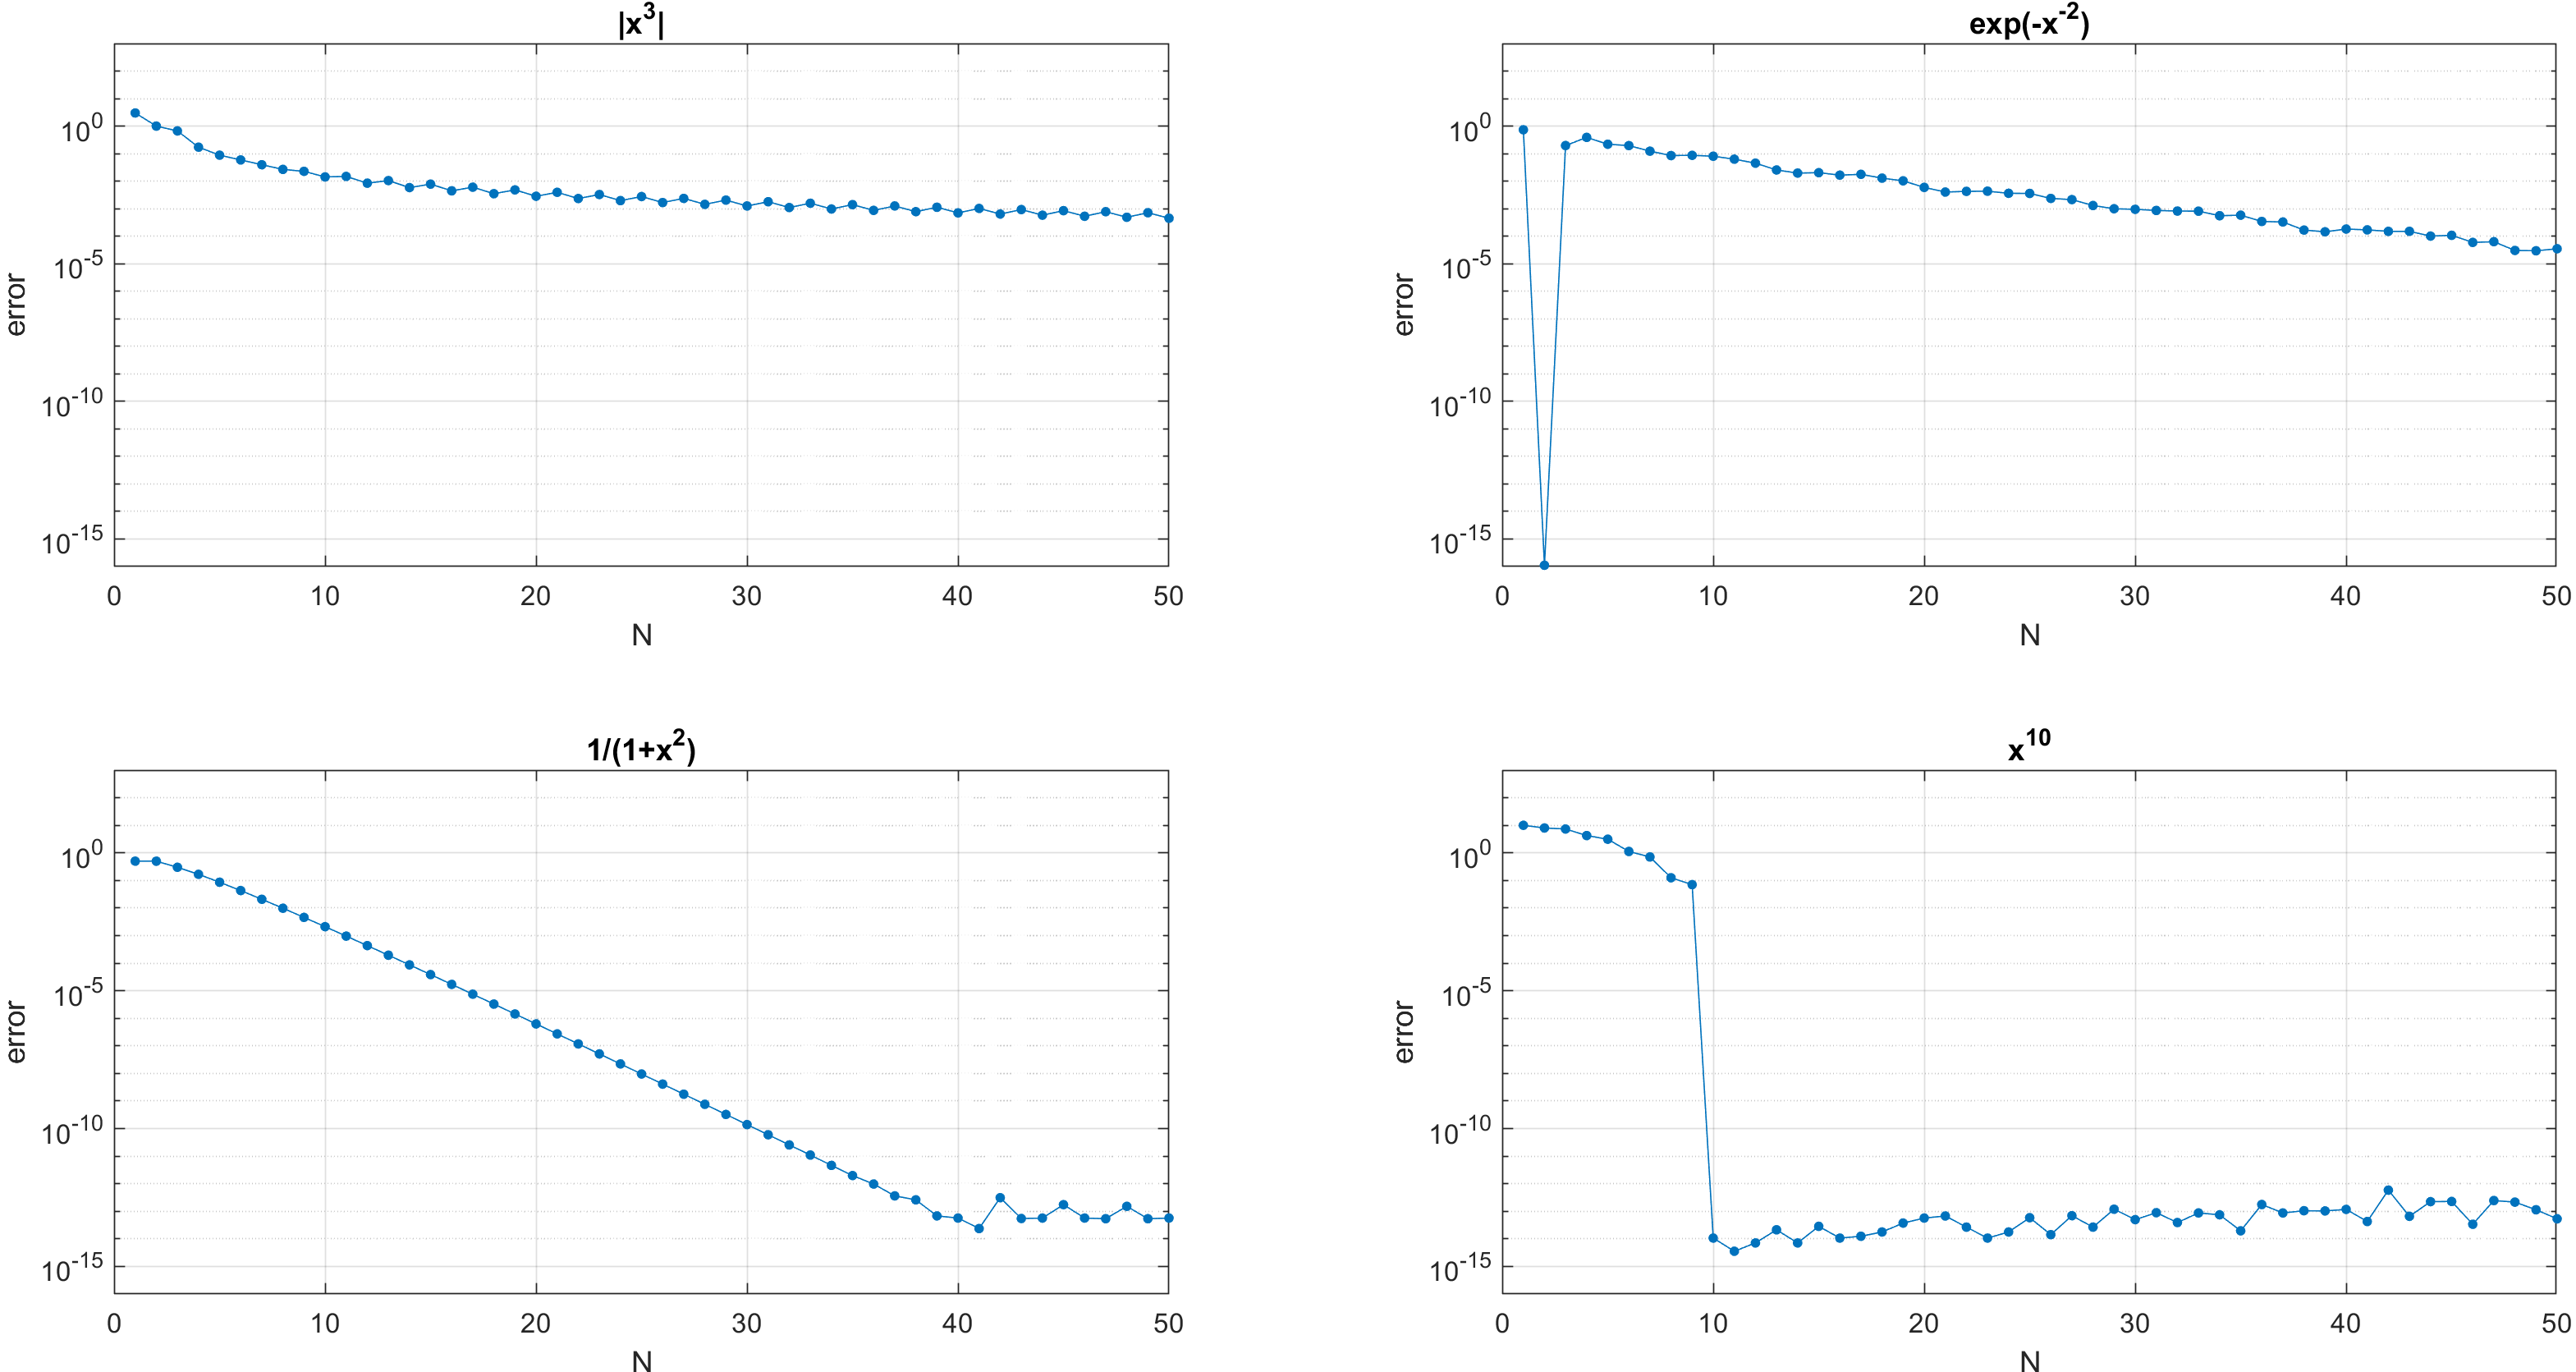
\includegraphics[scale=0.14]{8_3cheb.PNG}
\caption{cheb}
\end{figure}
\begin{figure}[htp]
\centering
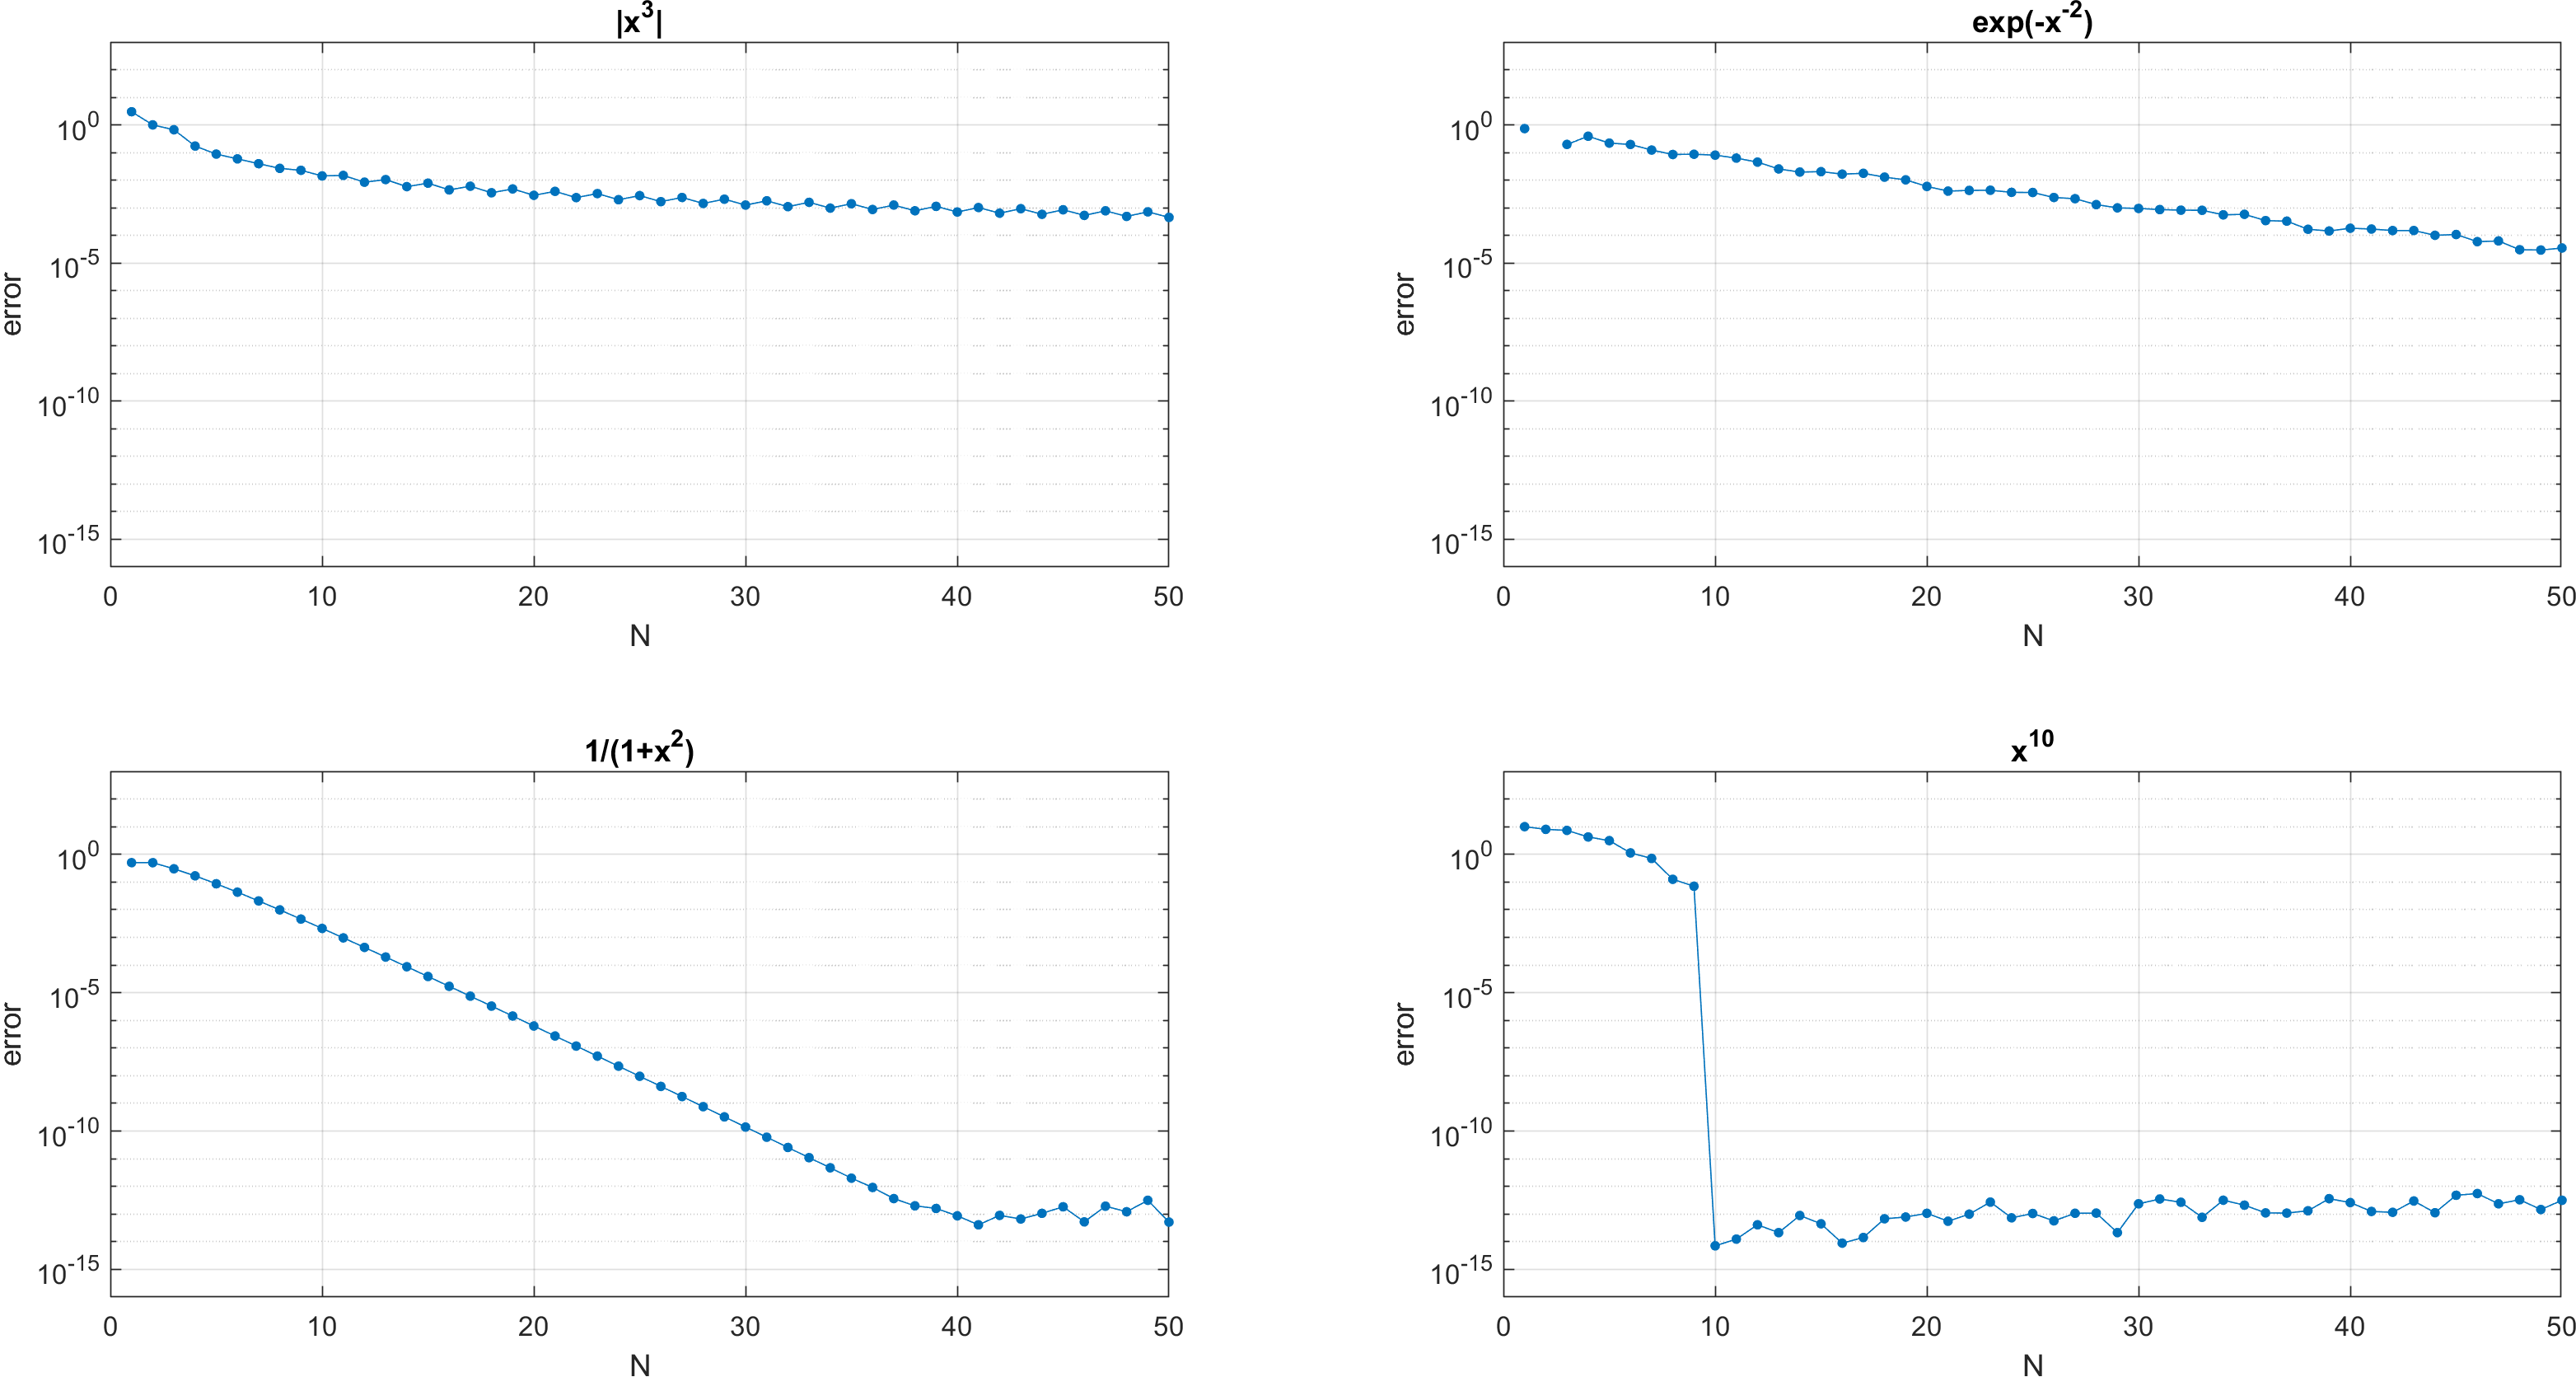
\includegraphics[scale=0.14]{8_3chebfft.PNG}
\caption{chebfft}
\end{figure}

We see that the round off error is the only difference between the two graphs. It can also be seen that the rounding error for the chebfft function is slightly less than that of the regular cheb function.

\newpage
\lstinputlisting{problem8_3.m}
\newpage

8.5. Write a code chebfft2 for second-order differentiation by the FFT, and show by examples that it matches the results obtained by matrices, apart from rounding errors.\\\\

Here, we used the functions $\sin(x), e^x,$ and $e^{-x^2}$ as examples to demonstrate the chebfft2 function. In order to write this function, all we needed to do is repeat the FFT, inverse FFT, and deriving the algebraic polynomial steps just on the derivative vector. So, we get the following graphs.\\

\begin{figure}[htp]
\centering
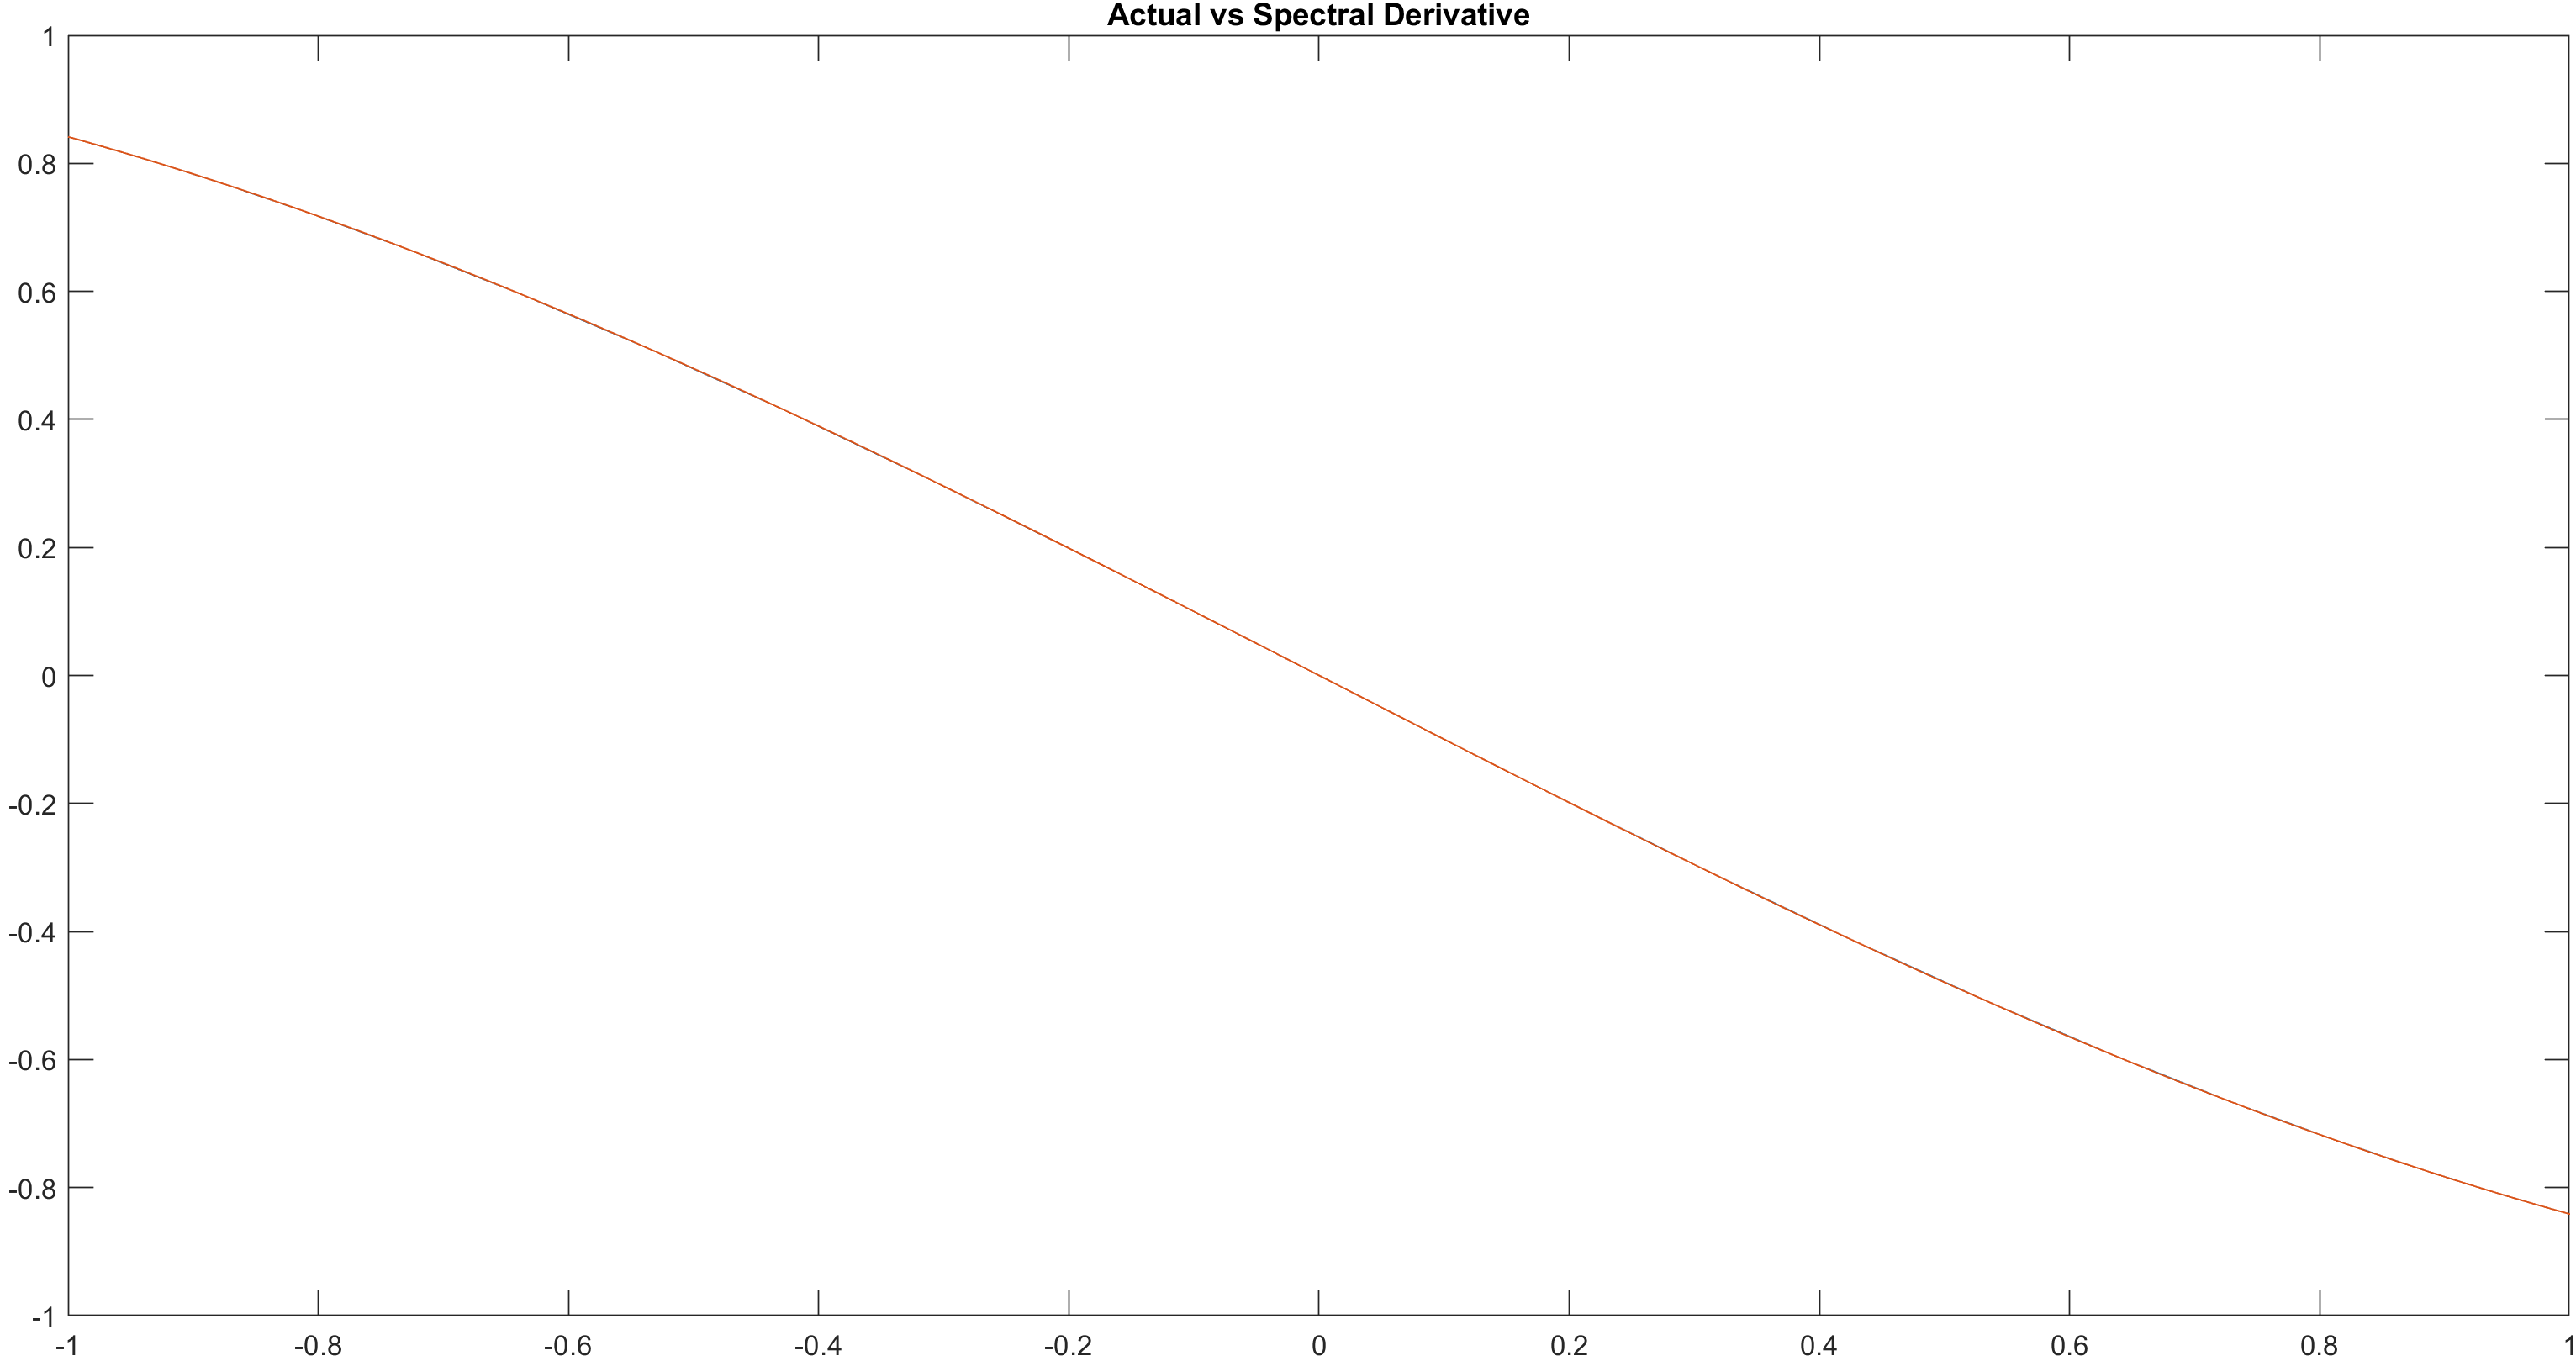
\includegraphics[scale=0.10]{8_5sin.PNG}
\caption{$\sin(x)$}
\end{figure}
\begin{figure}[htp]
\centering
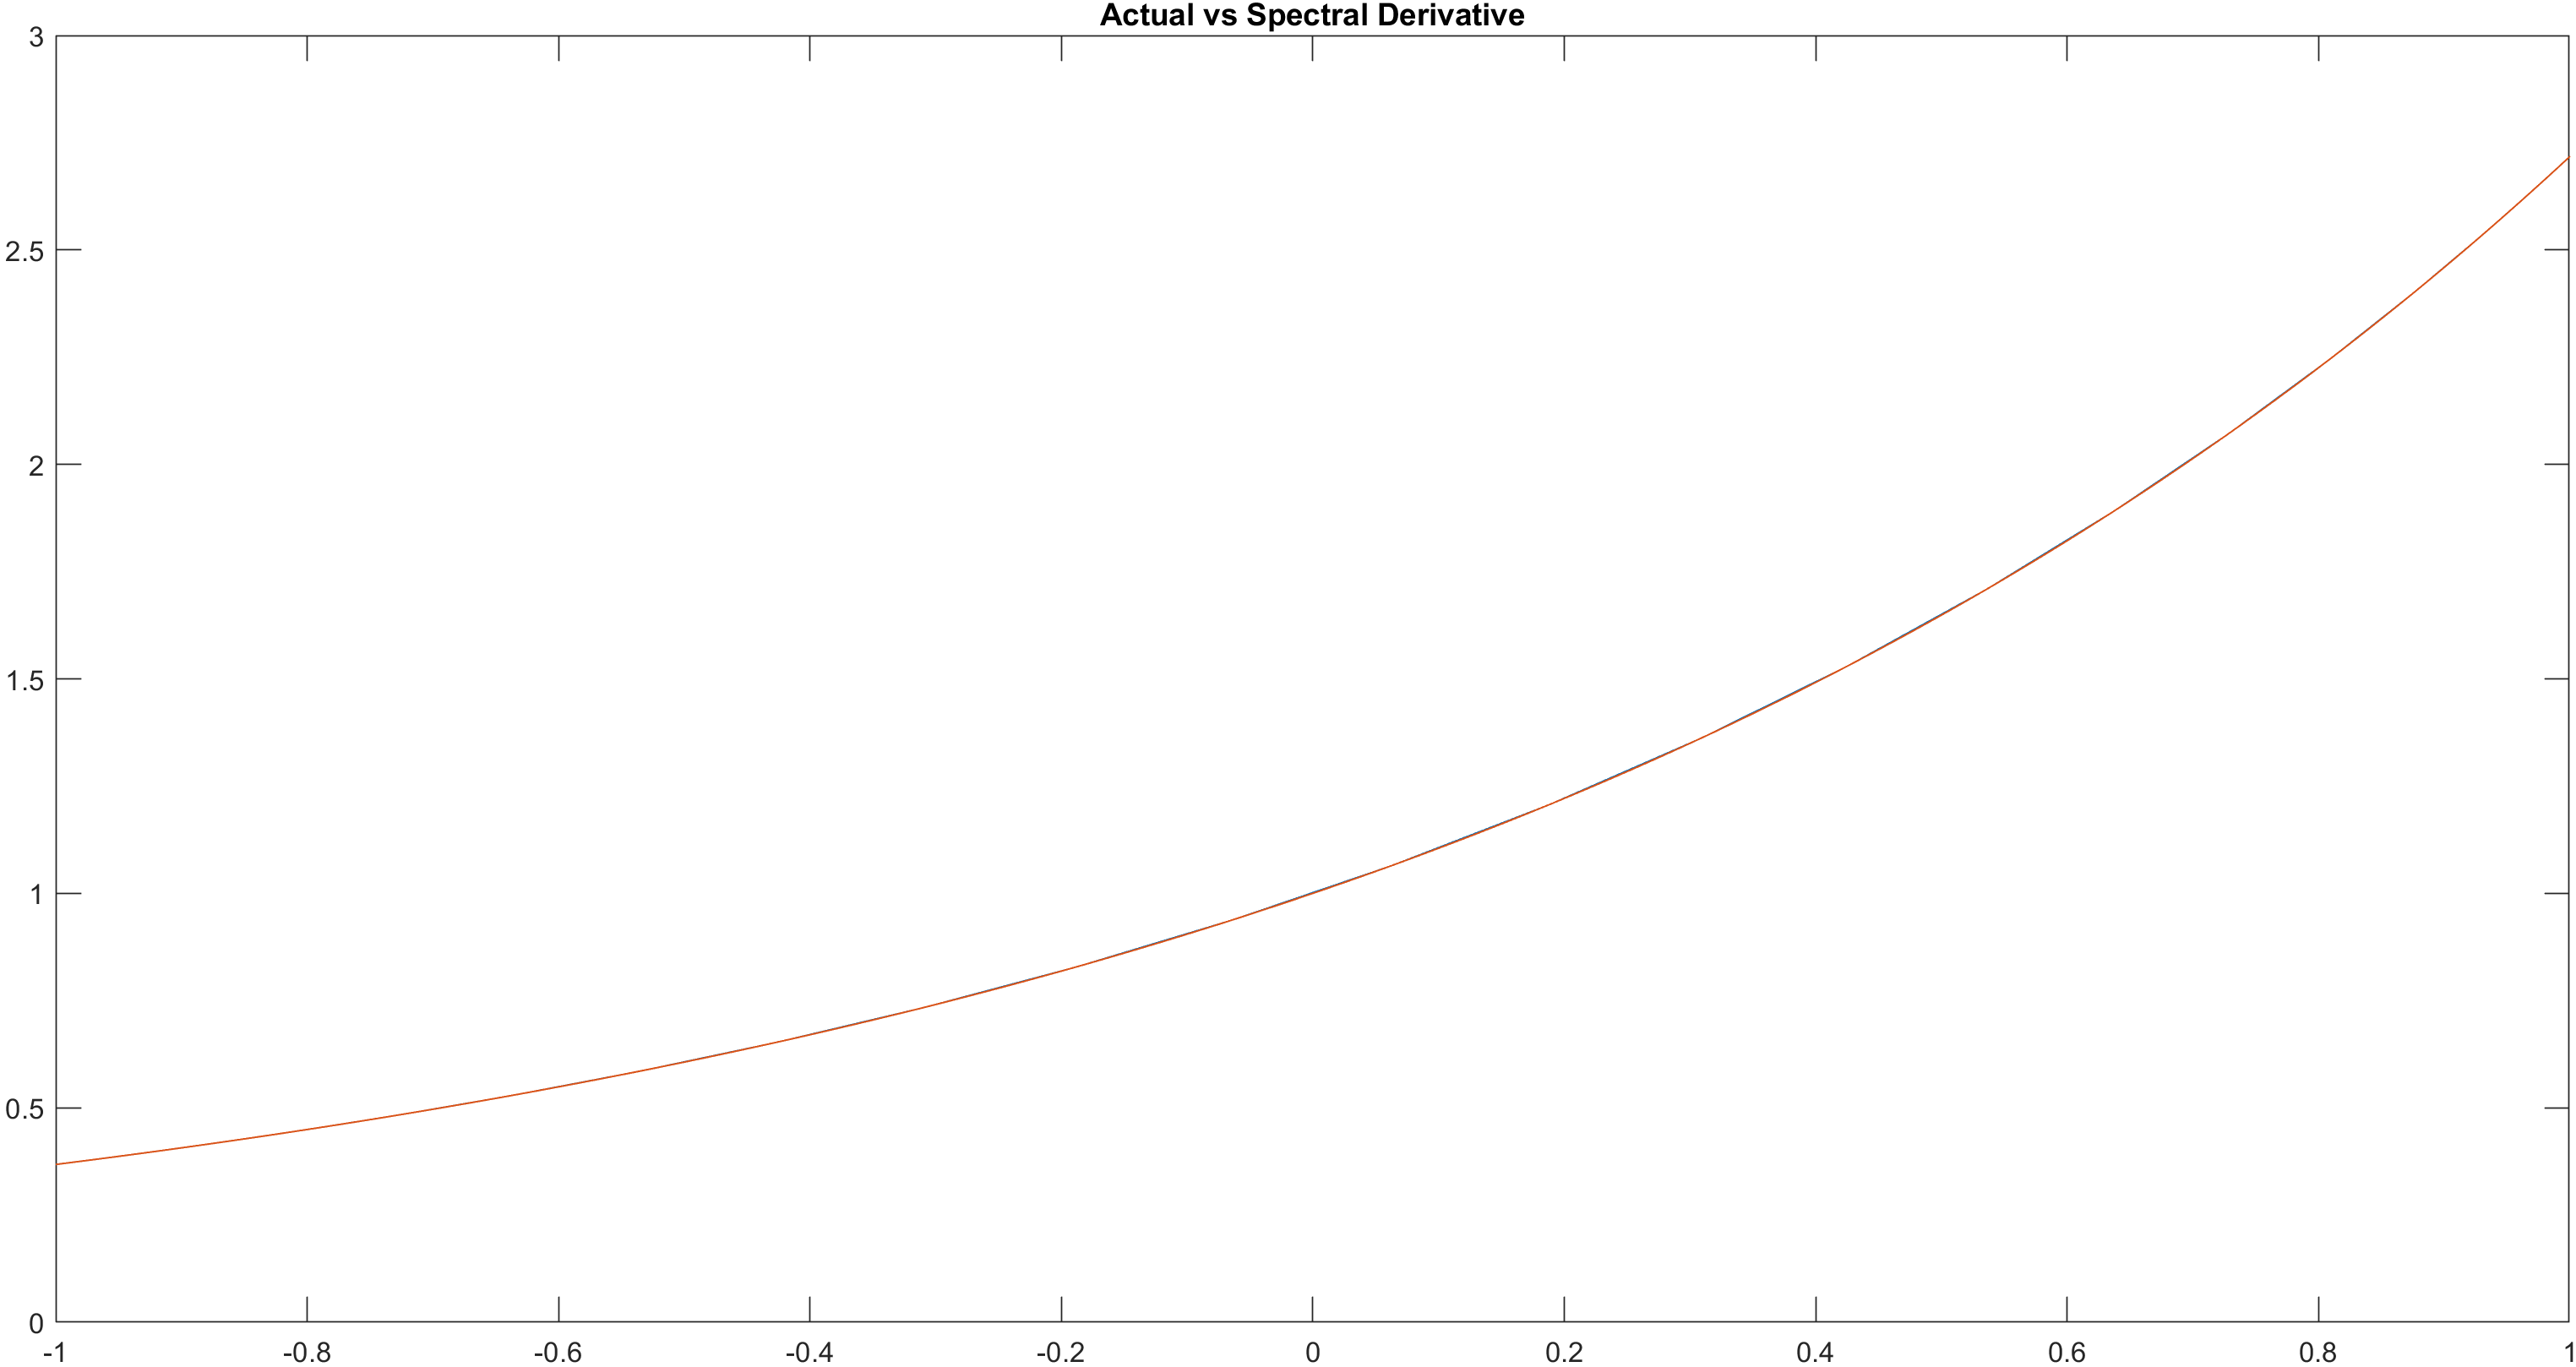
\includegraphics[scale=0.10]{8_5exp.PNG}
\caption{$e^x$}
\end{figure}
\begin{figure}[htp]
\centering
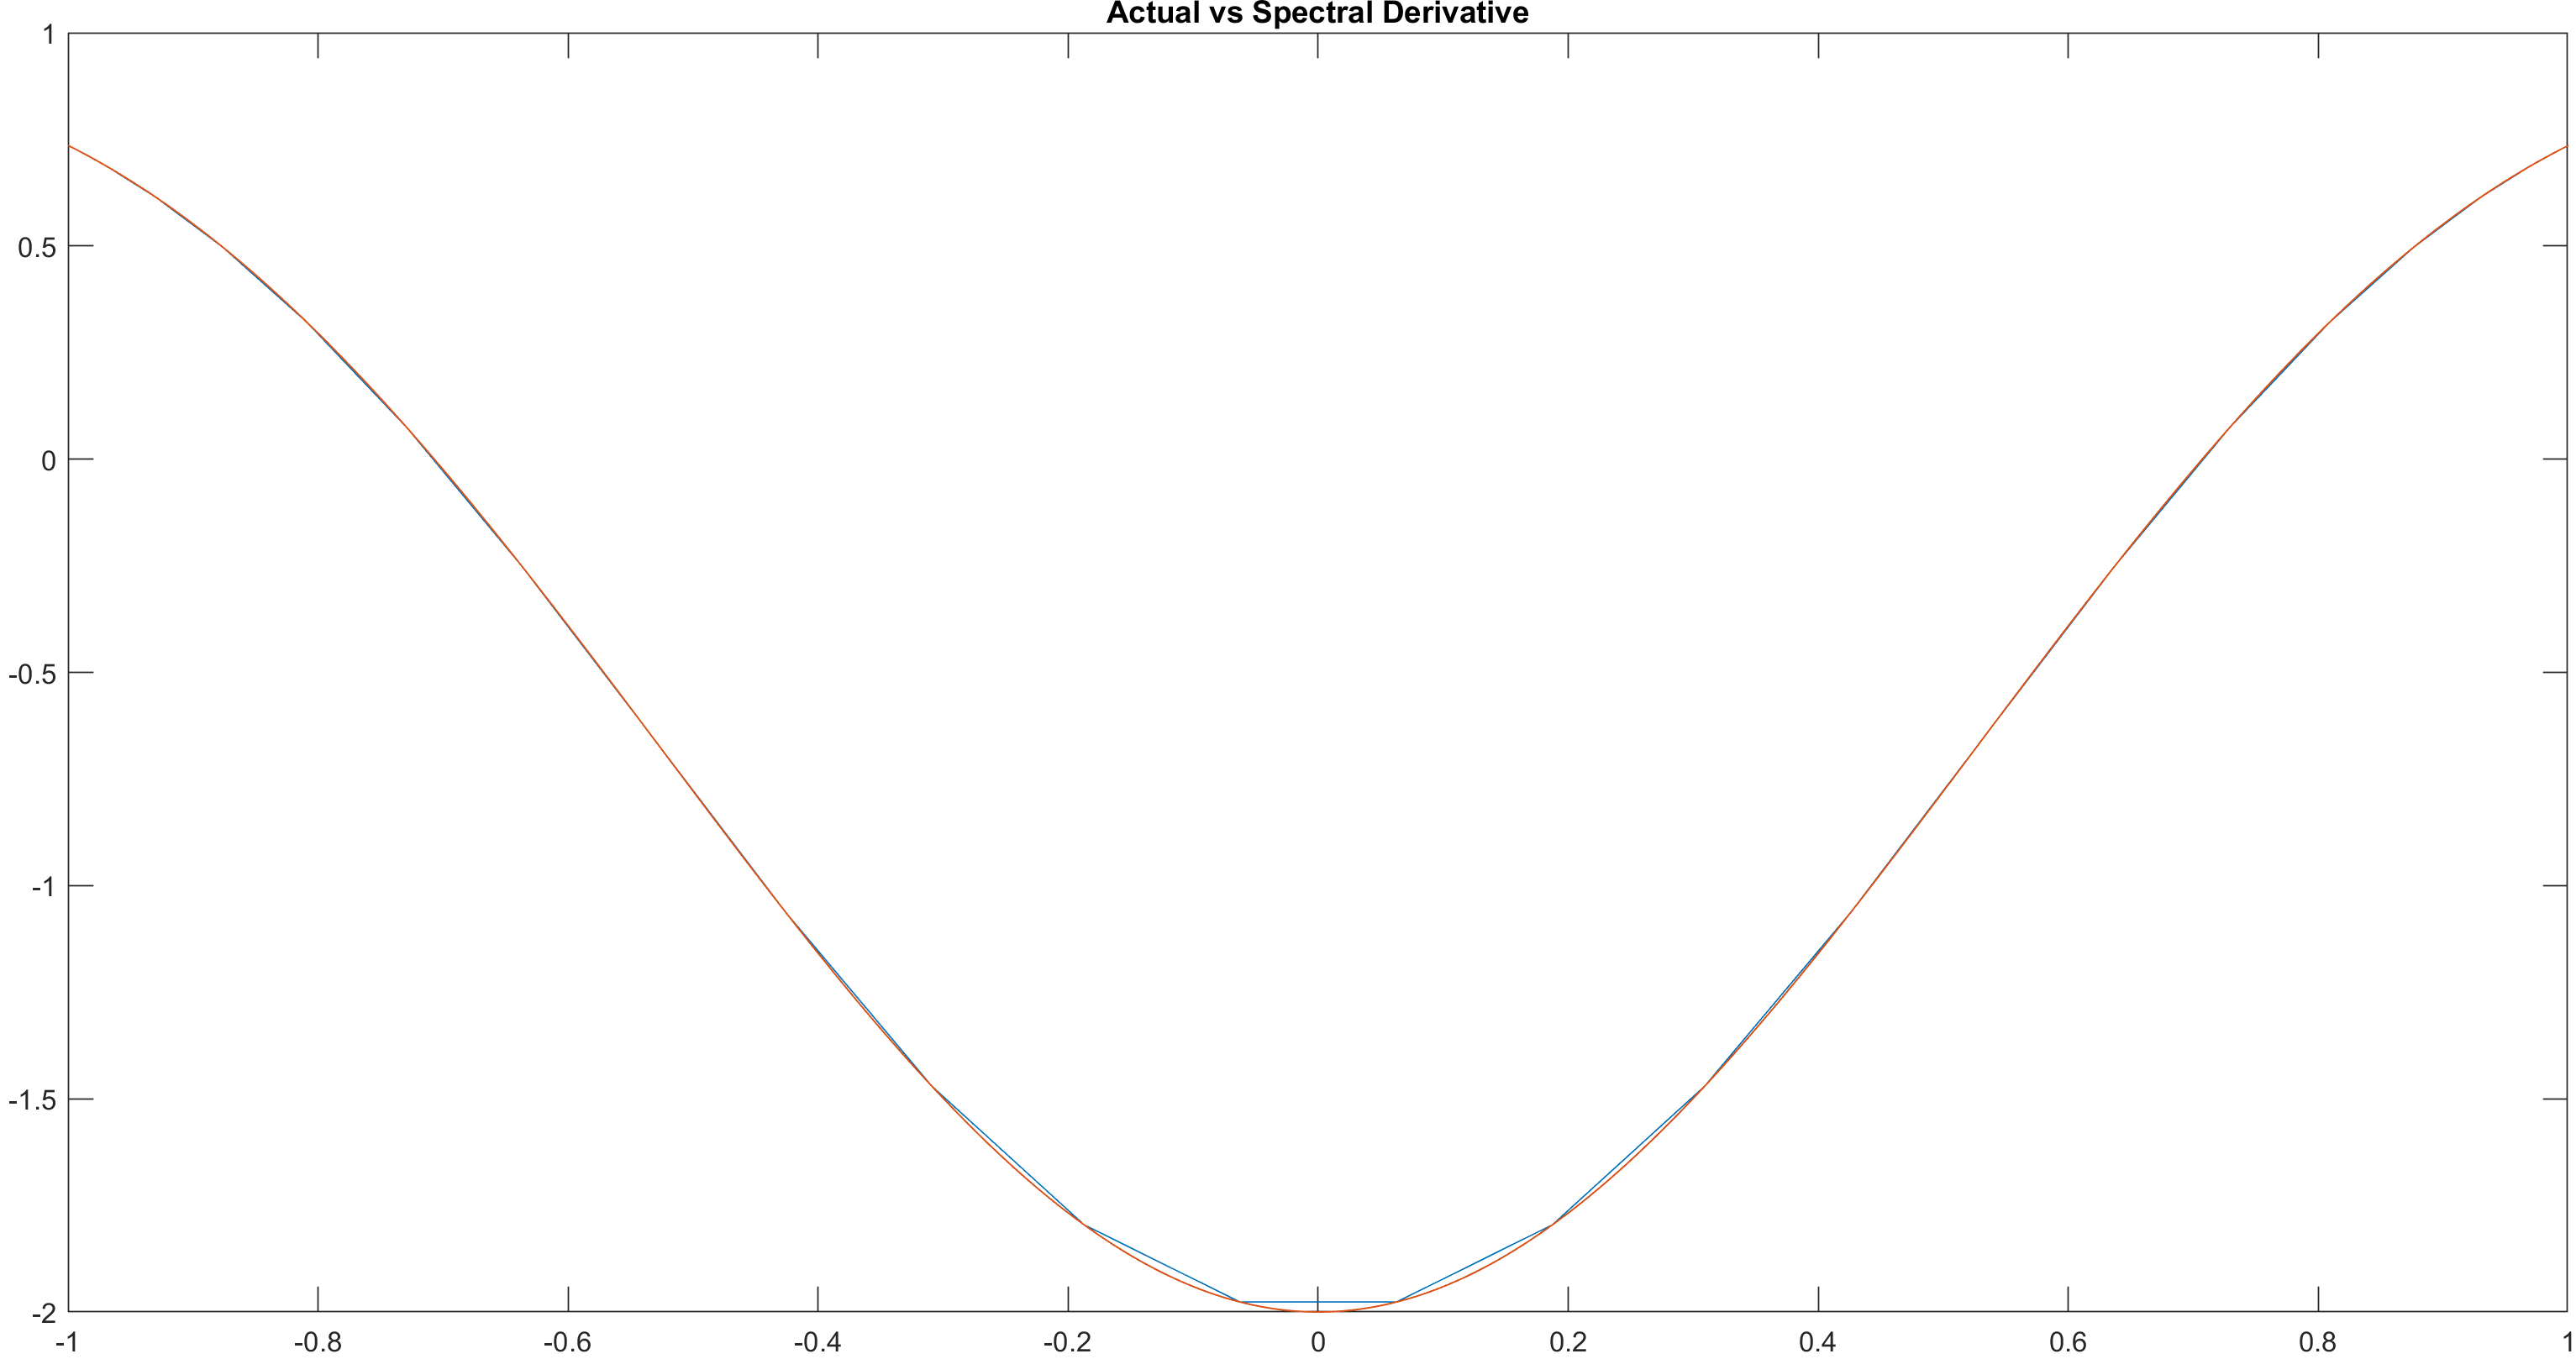
\includegraphics[scale=0.10]{8_5expx2.PNG}
\caption{$e^{-x^2}$}
\end{figure}

And we see that the matrices also provide the same outputs baring the roundoff errors.

\newpage
\lstinputlisting{problem8_5.m}






\end{document}